%%
%% This is file `sample-sigplan.tex',
%% generated with the docstrip utility.
%%
%% The original source files were:
%%
%% samples.dtx  (with options: `sigplan')
%% 
%% IMPORTANT NOTICE:
%% 
%% For the copyright see the source file.
%% 

%% Any modified versions of this file must be renamed
%% with new filenames distinct from sample-sigplan.tex.
%% 
%% For distribution of the original source see the terms
%% for copying and modification in the file samples.dtx.
%% 
%% This generated file may be distributed as long as the
%% original source files, as listed above, are part of the
%% same distribution. (The sources need not necessarily be
%% in the same archive or directory.)
%%
%% Commands for TeXCount
%TC:macro \cite [option:text,text]
%TC:macro \citep [option:text,text]
%TC:macro \citet [option:text,text]
%TC:envir table 0 1
%TC:envir table* 0 1
%TC:envir tabular [ignore] word
%TC:envir displaymath 0 word
%TC:envir math 0 word
%TC:envir comment 0 0
%%
%%
%% The first command in your LaTeX source must be the \documentclass command.
\documentclass[sigplan,screen]{acmart}
\usepackage{algorithm} 
\usepackage[noend]{algpseudocode} 
\usepackage[titles]{tocloft}
\usepackage{tikz}
\usepackage{listings}
\usepackage{xspace}
\usepackage{tcolorbox}
\usepackage{multirow}
\usepackage{adjustbox}
\usepackage[inline]{enumitem}
\usepackage{xspace}
\usepackage[listings,skins]{tcolorbox}
%\usepackage{subcaption}

\AtBeginDocument{%
  \providecommand\BibTeX{{%
    \normalfont B\kern-0.5em{\scshape i\kern-0.25em b}\kern-0.8em\TeX}}}

%% Rights management information.  This information is sent to you
%% when you complete the rights form.  These commands have SAMPLE
%% values in them; it is your responsibility as an author to replace
%% the commands and values with those provided to you when you
%% complete the rights form.
\setcopyright{acmcopyright}
\copyrightyear{2018}
\acmYear{2018}
\acmDOI{XXXXXXX.XXXXXXX}

%% These commands are for a PROCEEDINGS abstract or paper.
\acmConference[Conference acronym 'XX]{Make sure to enter the correct
  conference title from your rights confirmation emai}{June 03--05,
  2018}{Woodstock, NY}
%
%  Uncomment \acmBooktitle if th title of the proceedings is different
%  from ``Proceedings of ...''!
%
%\acmBooktitle{Woodstock '18: ACM Symposium on Neural Gaze Detection,
%  June 03--05, 2018, Woodstock, NY} 
\acmPrice{15.00}
\acmISBN{978-1-4503-XXXX-X/18/06}


%%
%% Submission ID.
%% Use this when submitting an article to a sponsored event. You'll
%% receive a unique submission ID from the organizers
%% of the event, and this ID should be used as the parameter to this command.
%%\acmSubmissionID{123-A56-BU3}

%%
%% For managing citations, it is recommended to use bibliography
%% files in BibTeX format.
%%
%% You can then either use BibTeX with the ACM-Reference-Format style,
%% or BibLaTeX with the acmnumeric or acmauthoryear sytles, that include
%% support for advanced citation of software artefact from the
%% biblatex-software package, also separately available on CTAN.
%%
%% Look at the sample-*-biblatex.tex files for templates showcasing
%% the biblatex styles.
%%

%%
%% The majority of ACM publications use numbered citations and
%% references.  The command \citestyle{authoryear} switches to the
%% "author year" style.
%%
%% If you are preparing content for an event
%% sponsored by ACM SIGGRAPH, you must use the "author year" style of
%% citations and references.
%% Uncommenting
%% the next command will enable that style.
%%\citestyle{acmauthoryear}


\makeatletter


\newenvironment{btHighlight}[1][]
{\begingroup\tikzset{bt@Highlight@par/.style={#1}}\begin{lrbox}{\@tempboxa}}
{\end{lrbox}\bt@HL@box[bt@Highlight@par]{\@tempboxa}\endgroup}


\definecolor{commentgreen}{RGB}{176, 176, 176}
\definecolor{rowcolor}{cmyk}{0,0.87,0.68,0.32}
\definecolor{rowcolor2}{cmyk}{ 20, 0, 37, 34}

\definecolor{eminence}{RGB}{108,48,130}
\definecolor{weborange}{RGB}{255,165,0}
\definecolor{frenchplum}{RGB}{129,20,82}
\definecolor{darkgreen}{RGB}{10, 92, 10}

\definecolor{celadon}{rgb}{0.67, 0.88, 0.69}
%\renewcommand{\blue}{}


% Subfigures caption


\newcommand\btHL[1][]{%
  \begin{btHighlight}[#1]\bgroup\aftergroup\bt@HL@endenv%
}
\def\bt@HL@endenv{%
  \end{btHighlight}%   
  \egroup
}
\newcommand{\bt@HL@box}[2][]{%
  \tikz[#1]{%
    \pgfpathrectangle{\pgfpoint{1pt}{0pt}}{\pgfpoint{\wd #2}{\ht #2}}%
    \pgfusepath{use as bounding box}%
    \node[anchor=base west, fill=orange!30,outer sep=0pt,inner xsep=1pt, inner ysep=0pt, rounded corners=3pt, minimum height=\ht\strutbox+1pt,#1]{\raisebox{1pt}{\strut}\strut\usebox{#2}};
  }%
}
\makeatother
\newcommand*\badge[1]{ \colorbox{red}{\color{white}#1}}
\newcommand{\tool}{Wasm-mutate\xspace}
\newcommand{\wasm}{Wasm\xspace}
\newcommand{\Wasm}{WebAssembly\xspace}
\newcommand{\etal}{et.al.\xspace}
\newcommand{\ie}{i.e.,\xspace}

\newtheorem{definition}{Definition}
\providecommand*{\definitionautorefname}{Definition}
\newtheorem{metric}{Metric}
\providecommand*{\metricautorefname}{Metric}

\newlistof{todo}{td}{List of TODOs}

\newcommand{\revision}[1]{{\textcolor{red}{#1}}}
\newcommand{\repourl}{\url{https://github.com/bytecodealliance/wasm-tools}}
\newcommand{\dataurl}{\url{https://github.com/Jacarte/tawasco}}

\newcommand*\step[1]{
\noindent\tikz[baseline=(char.base)]{
        \node[shape=circle,text=black,draw=black, fill=white,inner sep=1.2pt] (char) {#1};}}

\newcommand{\todo}[1]{%
\refstepcounter{todo}
\noindent\textbf{\badge{TODO}} {\color{red}#1}
\addcontentsline{td}{todo}
{\color{red}\thesection.\thetodo\xspace #1}}


\newcommand{\nick}[1]{%
\refstepcounter{todo}
\noindent\textbf{\badge{Nick}} {\color{red}#1}
\addcontentsline{td}{todo}
{\color{red}\thesection.\thetodo\xspace #1}}


% Define the WAT language
\lstdefinelanguage{WAT}{
    otherkeywords={},
    morekeywords=[1]{i32,f32,i64,f64,funcref, nop},
    morekeywords=[2]{0},
    morekeywords=[3]{add,or,const,mul,eqz,shl,get,rem_s,rem_u,ne,tee,sub,set,store},
    morekeywords=[4]{},
    morekeywords=[5]{global, get_global, mut, set_global, export, import,loop, memory, data, get_local,if,element, block,module, function, set_local,call,br_if,end,br, else, all,call_indirect,local,global,module, func, param, result, type, table, memory, elem},
    morekeywords=[6]{=,;},
    morekeywords=[7]{(,),[,],.},
    sensitive=false,
    morecomment=[l]{;},
    morecomment=[s]{;}{;},
    morestring=[b]",
    keywordstyle=[1]\color{eminence}\bfseries,
    keywordstyle=[3]\color{frenchplum},
    keywordstyle=[5]\color{darkgreen}\bfseries,
    commentstyle=\color{commentgreen}
}
\lstdefinestyle{nccode}{
        numbers=none,
        firstnumber=2,
        stepnumber=1,
        numbersep=10pt,
        tabsize=4, 
        showspaces=false,
        breaklines=true, 
        showstringspaces=false,
    %moredelim=**[is][\btHL]{`}{`},
    moredelim=**[is][{\btHL[fill=weborange!40]}]{`}{`},
    moredelim=**[is][{\btHL[fill=celadon!40]}]{!}{!}
}

\lstdefinestyle{WATStyle}{
  numbers=left,
  stepnumber=1,
  numbersep=10pt,
  tabsize=4,
  showspaces=false,
  showstringspaces=true,
}



\newcommand\tikzmarkWS[4]{%
\tikz[remember picture, overlay]{%
        \pgfusepath{use as bounding box}%
        \node[right=#3 mm, fill=white!0] at (1 mm,2 mm) (#1) {#2};
      %\node[right=#3 mm, align=center, shape=circle,text=black,draw=black, fill=white,inner sep=0.5pt] (#1) {#2};
  }
 }

  
 \newcommand\tikzmarkPROBE[4]{%
\tikz[remember picture, overlay]{%
        \pgfusepath{use as bounding box}%
        \node[right=#3 mm,text width=2mm,align =center,outer sep=0pt,inner xsep=1pt, inner ysep=0pt, rounded corners=3pt,anchor=north, minimum height=#4 mm, text depth = #4 mm] at (1 mm,2 mm) (#1) {};
      %\node[right=#3 mm, align=center, shape=circle,text=black,draw=black, fill=white,inner sep=0.5pt] (#1) {#2};
  }
 }

 % Replacement of the texttt command
 \lstdefinelanguage{ttt}{
    otherkeywords={},
    morekeywords=[1]{i32,f32,i64,f64,funcref,x,nop},
    morekeywords=[2]{0},
    morekeywords=[3]{container, add,const,mul,shl,get,rem_s,eqz,rem_u,ne,tee,sub,set,store,or},
    morekeywords=[4]{},
    morekeywords=[5]{global, get_global, mut, set_global, export, import,loop, memory, data, get_local,if, block,module, set_local,call,br_if,end,br, else, ret,all,call_indirect,local,global,module, func, param, result, type, table, (, ), memory, elem},
    morekeywords=[6]{=,;},
    morekeywords=[7]{[,],.},
    morekeywords=[8]{LHS, RHS, Cond},
    sensitive=false,
    morecomment=[l]{;},
    morecomment=[s]{;}{;},
    morestring=[b]",
    keywordstyle=[1]\color{eminence}\bfseries,
    keywordstyle=[3]\color{frenchplum},
    keywordstyle=[5]\color{darkgreen}\bfseries,
    keywordstyle=[7]\color{darkgreen}\bfseries,
    keywordstyle=[8]\color{frenchplum}\bfseries,
    keywordstyle=[2]\color{darkgreen}\bfseries,
    commentstyle=\color{commentgreen}
}
 \lstset{
    frameround=fttt,
    language=ttt,
    numbers=left,
    breaklines=true,
    basicstyle=\small\ttfamily
    }
 \renewcommand{\texttt}[1]{\lstinline{#1}}

 \lstdefinelanguage{TRACE}{
    otherkeywords={},
    morekeywords=[1]{dword, qword,ptr},
    morekeywords=[2]{0},
    morekeywords=[3]{mov, value, size, Writ, Read, I},
    morekeywords=[4]{rdx, ecx, r14},
    morekeywords=[5]{global, get_global, mut, set_global, export, import,loop, memory, data, get_local,if,element, block,module, function, set_local,call,br_if,end,br, else, all,call_indirect,local,global,module, func, param, result, type, table, memory, elem},
    morekeywords=[6]{=,;},
    morekeywords=[7]{(,),[,],.},
    sensitive=false,
    morecomment=[l]{;},
    morecomment=[s]{;}{;},
    morestring=[b]",
    keywordstyle=[1]\color{eminence}\bfseries,
    keywordstyle=[3]\color{frenchplum},
    keywordstyle=[5]\color{darkgreen}\bfseries,
    commentstyle=\color{commentgreen}
}

%%
%% end of the preamble, start of the body of the document source.
\begin{document}

%%
%% The "title" command has an optional parameter,
%% allowing the author to define a "short title" to be used in page headers.
\title{WebAssembly Binary Diversification with Guarantees}


%%
%% By default, the full list of authors will be used in the page
%% headers. Often, this list is too long, and will overlap
%% other information printed in the page headers. This command allows
%% the author to define a more concise list
%% of authors' names for this purpose.

%%
%% The abstract is a short summary of the work to be presented in the
%% article.
\begin{abstract}
This paper unveils \tool, an innovative, compiler-independent method for \Wasm software diversification. \tool, built atop an e-graph, encompasses 135 artfully designed rewriting rules catering to diversification from granular to broad levels. 
Our approach enables the generation of thousands of equivalent program variants within minutes. 
\tool excels in swiftly creating a vast array of unique, highly preserved \wasm programs, demonstrating significant variations in execution traces, including memory. 
Notably, \tool enhances the resilience of \wasm programs initially vulnerable to Spectre attacks, thereby offering a promising defensive strategy against such threats. 
Hence, \tool, with its contribution to the wider \wasm ecosystem, paves the way for safer and more robust \wasm applications.

\end{abstract}

%%
%% The code below is generated by the tool at http://dl.acm.org/ccs.cfm.
%% Please copy and paste the code instead of the example below.
%%
\begin{CCSXML}
\end{CCSXML}

%%
%% Keywords. The author(s) should pick words that accurately describe
%% the work being presented. Separate the keywords with commas.
\keywords{\Wasm, Software Diversification}

%% A "teaser" image appears between the author and affiliation
%% information and the body of the document, and typically spans the
%% page.

%%
%% This command processes the author and affiliation and title
%% information and builds the first part of the formatted document.
\maketitle

%%
%% The next two lines define the bibliography style to be used, and
%% the bibliography file.

\section{Introduction}


% Sota of Wasm
\Wasm has become the fourth official language of the web due to its low-level constructs that offer efficient execution times, significantly outpacing JavaScript \cite{haas2017bringing, WebAssemblyCoreSpecification}. 
Since its introduction in 2015, it has seen rapid adoption, with languages like Rust and C/C++ now being compiled to \wasm and run in all major browsers. 
Importantly, \wasm has also been adopted outside of browsers, with platforms like Fastly using it as a foundational technology \cite{fastly}.
In 2021, LLVM was responsible for generating 70\% of \Wasm binaries in use \cite{hilbig2021empirical}. However, the landscape is evolving with the introduction of new compilers that output \wasm binaries using methodologies distinct from LLVM. 
Examples include the Javy compiler, which packages JavaScript engine and code into a standalone \wasm \cite{javy}, and a recent development for Kotlin via the Kotlin Multiplatform framework\cite{kmm}. 
Consequently, \wasm to \wasm solutions are increasingly crucial, particularly in the context of software diversification.

% What is software diversification
Software diversification is a strategy that produces numerous variants of an original program, each retaining equivalent functionality while manifesting diverse execution behaviours \cite{cohen1993operating}. 
For \wasm, software diversification has been implemented directly within the LLVM compilation pipeline via superdiversification \cite{arteaga2020crow, MEWE}. 
However, such compiler dependant methods might restrict the benefits of diversification, particularly for emerging technologies that generate \wasm programs, as these may require the creation of specific compiler implementations. 
Software diversification carries numerous benefits, prominently enhancing automatic testing, malware evasion \cite{CABRERAARTEAGA2023103296}, and software protection. 
A salient example of its utility was the discovery of a CVE in Fastly in 2021 \cite{CVE}, achieved through the application of semantically equivalent transformations to a live deployed binary, thereby emphasizing the advantages of software diversification in testing scenarios.
In this paper, we propose a new compiler-agnostic approach for \Wasm software diversification, \tool.


% Wasm-mutate guanrantees are based on two aspects: manually verified rw and usage of components such as battle tested parsing and encoding.
\tool emerges as a \wasm to \wasm software diversification solution built on top of battle-tested parsing and encoding implementations used by the de facto backend \Wasm engine, wasmtime.
The heart of \tool consists of 135 carefully crafted rewriting rules, aiming diversification from fine to coarse grained levels. 
\tool in built on top of an e-graph data structure.
To the best of our knowledge, this work is pioneering in using an e-graph \cite{10.1145/3434304} for software diversification.
The strength of this technique lies in a characteristic property: every path through the e-graph represents a semantically equivalent variant of the input program. 
Following the previous property we enunciate a novel random e-graph traversal algorithm, which enables the generation of tens of thousands of equivalent variants from a single seed program in minutes.
Moreover, \tool is designed as a flexible framework that can be extended with additional rewriting rules as needed.
In our design process, we prioritized semantic equivalence, drawing insights from several well-established software diversification techniques. 
This includes the seminal work by Cohen et al. \cite{cohen1993operating}, which laid the foundation for our methodology.
\tool is poised to be a tool for testing \Wasm compilers and a suite of related tools, such as validators and interpreters. 
\tool stands to contribute to the broader \Wasm ecosystem, significantly bolstering software reliability. 
% What is wasm-mutate


%\todo{Next: talk about the protocol. How do we check behavioral diversity}
% Evaluation and hits to results
We evaluate the efficacy of \tool by quantifying the number of distinct and behaviorally diverse variants it can generate from a specified \wasm program. 
We draw on the original program corpus proposed by a diversification approach rooted in the LLVM compiler \cite{arteaga2020crow}, to provide the basis for our evaluation.
Our results show that \tool can rapidly create thousands of variants within an hour, including an impressive array of unique machine code variants generated by the wasmtime JIT compiler, cranelift. 
Intriguingly, these variants maintain their distinctiveness even when compiled into machine code by the same compiler.
To further analyze the behavior of these variants, we execute them using a wasmtime embedded engine. 
The results highlight considerable alterations in their execution traces.
To accentuate the practical utility of \tool, we employ it to generate diversified versions of \wasm programs known to be susceptible to Spectre attacks, as previously outlined in Swivel \cite{Swivel}. 
It generates variants for which the initial Spectre attacks are hardened.
Thus, \tool could serve as an effective strategy in the ongoing battle against Spectre and similar threats, providing an additional layer of security that supplements existing measures. 
The insights drawn from this study could potentially contribute to the development of more secure and resilient \Wasm applications.


To sum up, the contributions of this work are:

\begin{itemize}
    \item \tool, a versatile tool tailored for WebAssembly to WebAssembly software diversification, \repourl
    \item Empirical evidence on static and dynamic differences provided by the variants created by \tool.
    \item Empirical evidence on how \tool can protect cache timing side-channel attacks, specifically, Spectre.
    
\end{itemize}

This paper is structured as follows. 
In \autoref{background}, we introduce WebAssembly, the concepts of semantic equivalence and what we state as a rewriting rule.
In \autoref{tech}, we explain and detail the architecture and implementation of \tool.
We formulate our research questions in \autoref{eval}, answering them in \autoref{results}.
We discuss open challenges related to our research in \autoref{discussion}, in order to help future research projects on similar topics.
In \autoref{rw} we highlight works related to our research on software diversification.
We finalize with our conclusions \autoref{conc}.

\section{Background}
\label{background}

In this section, we define and formulate the foundation of this work: WebAssembly and its runtime structure, semantic equivalence modulo input, rewriting rules and e-graphs.
Along with the paper, we use the terms, metrics and concepts defined here.

\subsection{WebAssembly}

WebAssembly (Wasm) is a binary instruction set initially  meant for the web, and now also used in the backend. 
It was adopted as a standardized language by the W3C in 2017, building upon the work of Haas et al. \cite{haas2017bringing}. One of Wasm's primary advantages is that it defines its own Instruction Set Architecture (ISA), which is both platform-independent. As a result, a Wasm binary can execute on virtually any platform, including web browsers and server-side environments. 
WebAssembly programs are compiled ahead-of-time from source languages such as C/C++, Rust, and Go, utilizing compilation pipelines like LLVM. 



\lstdefinestyle{watcode}{
  numbers=none,
  stepnumber=1,
  numbersep=10pt,
  tabsize=4,
  showspaces=false,
  breaklines=true, 
  showstringspaces=false,
  moredelim=**[is][{\btHL[fill=black!10]}]{`}{`},
  moredelim=**[is][{\btHL[fill=celadon!40]}]{!}{!}
}
{
%\captionsetup{width=0.9\linewidth}
\lstset{
  language=WAT,
  style=watcode,
  breaklines=true, 
  basicstyle=\footnotesize\ttfamily,
  %numberstyle=\footnotesize,
  numbersep=2.5pt,
  %firstnumber=1,
  escapeinside={``},
  %numbers=left,
  %postbreak=\mbox{\textcolor{red}{$\hookrightarrow$}\space},
  }
    \begin{lstlisting}[label=example:wasmprogram,caption={Simplified WebAssembly code for the program of \autoref{example:cprogram}.}, captionpos=b]{Name}
(module
  (@custom "producer" "llvm.." )
  (import "env" "println" (func $println (param i32)))
  (memory 1)
  (export "memory" (memory 0))
  (func $main
    (local $sum i32)
    (local $i i32)
    (local $arr_offset i32)
    ; Initialize sum to 0 ;
    i32.const 0
    local.set $sum
    ; Initialize arr_offset to point to start of the array in memory ;
    i32.const 0
    local.set $arr_offset
    ; Initialize the array in memory;
    i32.const 0
    i32.const 1
    i32.store
    ...
    i32.store
    ...
    loop
      local.get $i
      i32.const 5
      i32.lt_s
      if
        ; Load array[i] and add to sum ;
        local.get $arr_offset
        local.get $i
        ...
        ; Increment i ;
        local.get $i
        i32.const 1
        i32.add
        local.set $i
        br 0
      else
        ; End loop ;
        i32.const 0
      end
    end
    
    ; Call external function to print sum ;
    local.get $sum
    call $println
  )
  ; Start the main function ;
  (start $main)
  )
\end{lstlisting}
}


% We do not enumerate the types, lets try to be as much agnostic to the version of Wasm as possible
WebAssembly programs operate on a virtual stack that allows primitive data types.
% These same data types are used to annotate instructions in the WebAssembly code.
Additionally, a WebAssembly program might include several custom sections.
For example, binary producers such as compilers use custom sections to store metadata, such as the name of the compiler that generates the Wasm code.
A WebAssembly program also declares memory sections and globals, which are used to store, manipulate and share data during program execution, e.g. to share data with the host engine of the WebAssembly binary.

WebAssembly is designed with isolation as a primary consideration. For instance, a WebAssembly binary cannot access the memory of other binaries or cannnot interact directly with browser's APIs, such as the DOM or the network. Instead, communication with these features is constrained to functions imported from the host engine, ensuring a secure and safe Wasm environment.
Moreover, control flow in WebAssembly is managed through explicit labels and well-defined blocks, which means that jumps in the program can only occur inside blocks, unlike regular assembly code \cite{10.1145/3062341.3062363}. 
%\todo{Change the example to Rust}
In \autoref{example:cprogram}, we provide an example of a C program that contains a function declaration, a loop, a loop conditional, and a memory access. When the C code is compiled to WebAssembly, it produces the code shown in \autoref{example:wasmprogram}. The stack operations are folded with parentheses.
The module in the example contains the components described previously.

% Now we talk a bit about what is the state of a Wasm program.
%\todo{The following text should be revised. }

The WebAssembly runtime structure is described in the WebAssembly specification and it includes 10 key elements: the Store, Stack, Locals, Module Instances, Function Instances, Table Instances, Memory Instances, Global Instances, Export Instances, and Import Instances. These components interact during the execution of a WebAssembly program, collectively defining the state of a program during its runtime.

Two of these elements, the Stack and Memory instances, are particularly significant in maintaining the state of a WebAssembly program during its execution. The Stack holds both values and control frames, with control frames handling block instructions, loops, and function calls. Meanwhile, Memory Instances represent the linear memory of a WebAssembly program, consisting of a contiguous array of bytes.
In this paper, we highlight the aforementioned two components to define, compare and validate the state of two Wasm programs during their execution. 

\subsection{Semantic Equivalence}

Semantic equivalence refers to the notion that two programs or functions are considered equivalent if, for a given specified input domain, they produce the same output values or have the same observable behavior \cite{10.1145/2594291.2594334}. 
In other words, the semantics of the two programs are equivalent when the input-output relationship (w/ possibly some abstraction), even if the internal implementation details or the structure of the programs differ.


Let us illustrate this with an example.
Assume two programs $P$ and $P'$ (\autoref{example:state1} and \autoref{example:state2} respectively) where $P'$ is the result of modifying a code in the first instruction of its unique function.
The program $P'$ has two extra instructions right before returning from the function.
The remaining components of the original binary are not modified.



\lstdefinestyle{watcode}{
  numbers=none,
  stepnumber=1,
  numbersep=10pt,
  tabsize=4,
  showspaces=false,
  breaklines=true, 
  showstringspaces=false,
    moredelim=**[is][{\btHL[fill=weborange!40]}]{`}{`},
    moredelim=**[is][{\btHL[fill=celadon!40]}]{!}{!}
}
   \begin{minipage}[t]{0.45\linewidth}
    \lstset{
        language=WAT,
                        style=watcode,
        basicstyle=\footnotesize\ttfamily,
                        columns=fullflexible,
                        breaklines=true}
        
        \begin{lstlisting}[label=example:state1,caption={Program P.},frame=b, captionpos=b]{state1}
func (;0;) (type 0) (param i32 f32) (result i64)
    i64.const 1
        \end{lstlisting}
\end{minipage}\hfill
\begin{minipage}[t]{0.45\linewidth}
    \lstset{
        language=WAT,
                        style=watcode,
        basicstyle=\footnotesize\ttfamily,
                        columns=fullflexible,
                        breaklines=true}
        
        \begin{lstlisting}[label=example:state2,caption={Program $P'$, transformation of program $P$.},frame=b, captionpos=b]{state2}
func (;0;) (type 0) (param i32 f32) (result i64)
    i64.const 1
    !i32.const 42!
    !i32.drop!
        \end{lstlisting}
\end{minipage}


The state of the program $P$ when entering the function is its stack $[S]$, 
the program $P'$ has the same state before executing the function.
The input values of the function for both programs are $L$, their outputs are the top of the stack at the end of the execution.


Program $P$ has the state $[[S:i32.const\ 1]]$ just before returning from the function execution.
When we trace the states of the program $P'$, we can construct the following sequence of states:
\begin{enumerate}
    \item $[[S: i32.const\ 1]]$ the integer constant 1 is now on the top of the stack.
    \item $[[S: i32.const\ 1, i32.const\ 42]]$ the integer constant 32 is  the top of the stack.
    \item $[[S: i32.const\ 1]]$ the top of the stack is dropped. The function execution stops.
\end{enumerate}
Notice that, the stack state of program $P'$ is the same as program $P$.
Thus, we can say that these two programs are semantically equivalent.
Even though the programs share semantic equivalence, they display differences during execution. 
Specifically, $P'$ stresses more on the stack by adding and subsequently dropping more values.
These subtle yet significant differences form the crux of the diversification approaches discussed in this study.






\subsection{Rewriting rule}
\label{rewriting}

Our definition of a rewriting rule draws from the one proposed by Sasnauskas et al. \cite{2017arXiv171104422S}, and integrates a predicate to specify the replacement condition.
Concretely, a rewriting rule is defined as a tuple, denoted as \texttt{(LHS, RHS, Cond)}. Here, \texttt{LHS} refers to the code segment slated for replacement, \texttt{RHS} is the proposed replacement, and \texttt{Cond} stipulates the conditions under which the replacement is acceptable.
Importantly, \texttt{LHS} and \texttt{RHS} are meant to be semantically equivalent, per the definition of previous section.


For example, the rewriting rule \texttt{(x,\ x\ i32.or\ x, \{\})} implies that the \texttt{LHS} 'x' is to be replaced by an idempotent bitwise \texttt{i32.or} operation with itself, absent any specific conditions.
Notice that, for this specific rule, the commutative property shared by \texttt{LHS} and \texttt{RHS}, symbolized as \texttt{(LHS, RHS) = (RHS, LHS)}.
Besides, the \texttt{Cond} element could be an arbitrary criterion. 
For instance, the condition for applying the aforementioned rewriting rule could be to ensure that the newly created binary file does not exceed a threshold binary size.

Based on our understanding, our research is the first to apply the concept of rewriting rules to WebAssembly.
This will expand the potential use cases of wasm-mutate. 
Beyond its role as a diversification tool, it can also be used as a standard tool for conducting program transformations in WebAssembly.


\section {Design of Wasm-Mutate}
\label{tech}
% Here is the state of wasm-mutate \url{https://github.com/bytecodealliance/wasm-tools/issues/415}.

In this section we present \tool, a novel technique to diversify
WebAssembly binaries and produce semantically equivalent variants.

\begin{figure*}[h!]
    \centering
    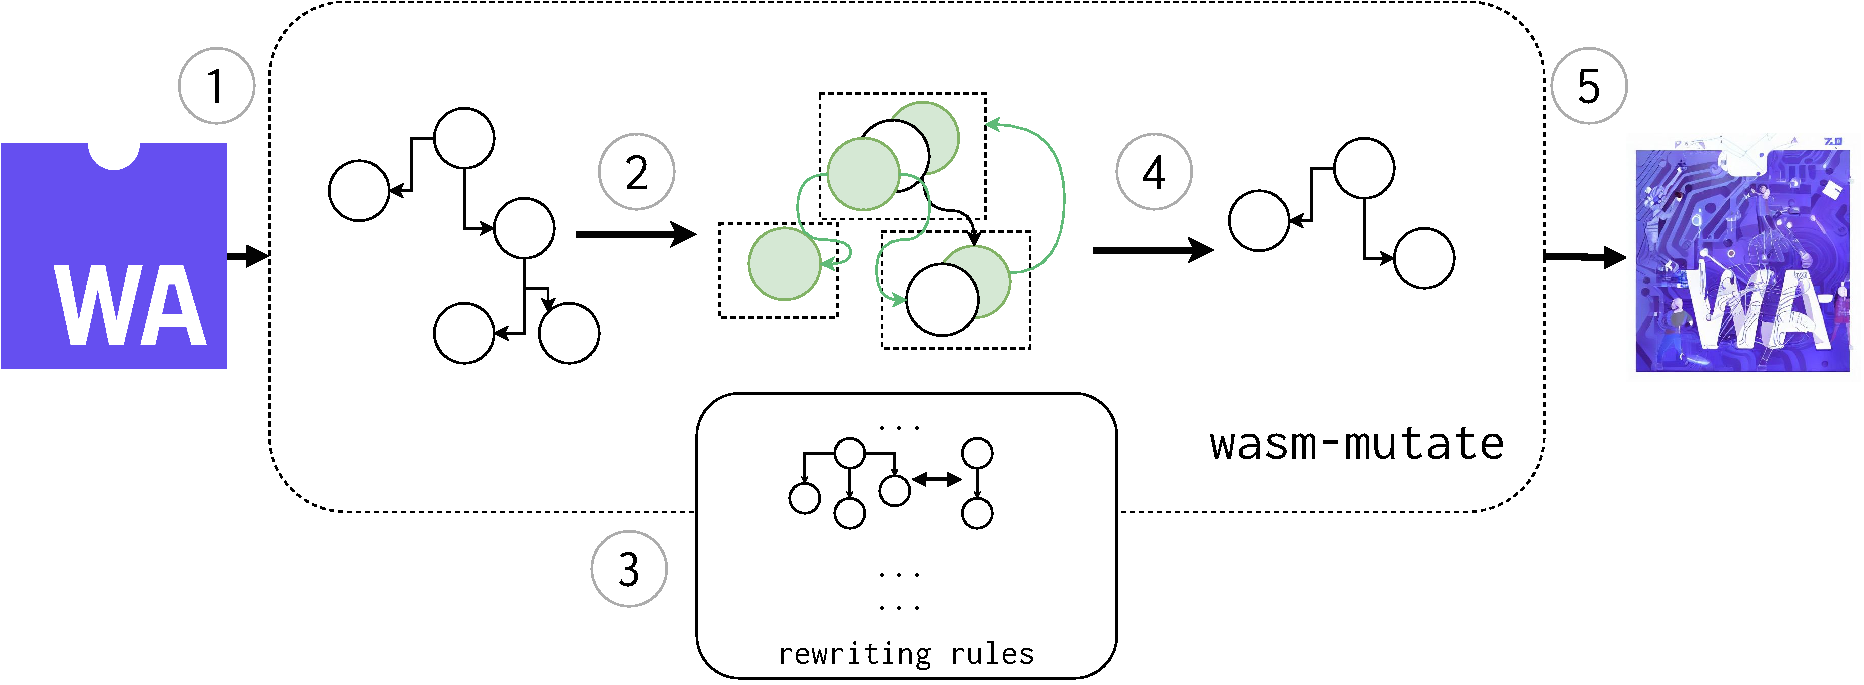
\includegraphics[width=0.8\linewidth]{figures/wasm-mutate-general.pdf}
    \caption{ \tool workflow and high level architecture.}
  \label{fig:wasm-mutate}
\end{figure*}

\subsection{Overview}
The primary objective of \tool is to perform WebAssembly to WebAssembly diversification, i.e., generate semantically equivalent variants from a given WebAssembly binary input. 
\tool's central approach involves synthesizing these variants by substituting parts of the original binary using rewrite rules. 
It leverages a comprehensive set of rewrite rules, boosted by a proposed random traversals of e-graph structures (refer to \autoref{alg}).


In \autoref{fig:wasm-mutate} we illustrate the workflow of \tool: it starts with a WebAssembly binary as its input \step{1}.
It parses the original binary \step{2}, turning the input program into tree abstractions, i.e., \tool builds the control flow graph and data flow graph. 
Using the defined rewriting rules, \tool builds an e-graph \step{3} for the original program.
Parts of the original program are randomly replaced by traversal of the e-graph \step{4}.
The outcome of \tool is a semantically equivalent variant of the original binary \step{5}.
The tool guarantees semantically equivalent variants because each individual rewrite rule is semantic preserving.
Notice that, the output result in step \step{5} can be connected again to step \step{1}, enabling the stacking of multiple transforms with several iterations of \tool. 


\subsection{WebAssembly Rewriting rules}
%\todo{ideally one citation per transformation, we do not want to claim novelty on any of them, we claim novelty on the e-graph / integration part}

% 
\lstdefinestyle{watcode}{
  numbers=none,
  stepnumber=1,
  numbersep=10pt,
  tabsize=4,
  showspaces=false,
  breaklines=true, 
  showstringspaces=false,
    moredelim=**[is][{\btHL[fill=weborange!40]}]{`}{`},
    moredelim=**[is][{\btHL[fill=celadon!40]}]{!}{!},
    moredelim=**[is][{\btHL[fill=frenchplum!40]}]{bb}{bb},
    moredelim=**[is][{\btHL[fill=eminence!40]}]{bc}{bc}
}



\lstset{
        language=WAT,
        style=watcode,
        basicstyle=\footnotesize\ttfamily,
        columns=fullflexible,
        breaklines=true}




\begin{table*}
\renewcommand\arraystretch{1.1}
\begin{adjustbox}{width=\textwidth,totalheight=\textheight, keepaspectratio}
    \begin{tabular}{p{0.15\textwidth} | p{0.45\textwidth} |p{0.45\textwidth} | p{0.03\textwidth}}
        \hline
        Name & Original & Replacement & Level \\
        \hline \hline

        Add \texttt{type} 
%&  
\vspace{-4mm}
\begin{lstlisting}[numbers=none]{Name}
(module
  (type (;0;) (func (param i32) (result i64)))
        \end{lstlisting}   
%&  
%\vspace{-4mm}
LHS
\begin{lstlisting}[numbers=none]{Name}
(module
  (type (;0;) (func (param i32) (result i64)))
!+ (type (;0;) (func (param i64) (result i32 i64)))!
        \end{lstlisting}  
\hrulefill

RHS
\begin{lstlisting}[numbers=none]{Name}
(module
  (type (;0;) (func (param i32) (result i64)))
!+ (type (;0;) (func (param i64) (result i32 i64)))!
        \end{lstlisting}   
 %       \vspace{-4mm}
%&   S \\

%& \multicolumn{3}{l}{
%\begin{minipage}{0.9\textwidth}

    %\begin{tcolorbox}[boxrule=0.1pt,arc=.1em,boxsep=-1.5mm]
    %    \textbf{Guarantees:} The generated type is not duplicated. Recalculates type indexes. Notice that the new type is used during the compilation of the binary and not during runtime. Therefore, we can say that the state of the new program is the same as the original at any moment of its execution.
    %\end{tcolorbox}
%\end{minipage}
%} \\
%&
%$[St, S, L, Mi, Fi, Ti, M, G, E, I]$ &
%$[St, S, L, Mi, Fi, Ti, M, G, E, I]$ \\
%\hline
        
        Add \texttt{function} 
&  
        \vspace{-4mm}
\begin{lstlisting}[numbers=none]{Name}
 (module
  (type (;0;) (func (param i32 f32) (result i64)))
        \end{lstlisting}   
&  
        \vspace{-4mm}
\begin{lstlisting}[numbers=none]{Name}
 (module
  (type (;0;) (func (param i32 f32) (result i64)))
!+(func (;0;) (type 0) ...!
!+   i64.const 0) !
        \end{lstlisting}  
        \vspace{-4mm}
&   S \\
%& \multicolumn{3}{l}{
%\begin{minipage}{0.9\textwidth}

    %\begin{tcolorbox}[boxrule=0.1pt,arc=.1em,boxsep=-1.5mm]
   %     \textbf{Guarantees:} At the end of the transformation, the type of the function is defined in the type index. The body of the function is correct regarding the state of the stack. \tool recalculates the indexes for the functions of the binary. The added function is not included as a call in the new program. Therefore, during the execution of the program, its state is the same. Thus, the new program is semantically equivalent to the first one.
    %\end{tcolorbox}
%\end{minipage}
%} \\
%&
%$[St, S, L, Mi, Fi, Ti, M, G, E, I]$ &
%$[St, S, L, Mi, Fi, Ti, M, G, E, I]$ \\
\hline

        
        Remove \texttt{function} 
&  
        \vspace{-4mm}
\begin{lstlisting}[numbers=none]{Name}
`- (module (import "" "" (func)))`
        \end{lstlisting}   
&  
        \vspace{-4mm}
\begin{lstlisting}[numbers=none]{Name}
 (module (type (func)))

        \end{lstlisting}  
        \vspace{-4mm}
&   S \\
%& \multicolumn{3}{l}{
%\begin{minipage}{0.9\textwidth}

%    \begin{tcolorbox}[boxrule=0.1pt,arc=.1em,boxsep=-1.5mm]
%        \textbf{Guarantees:} All functions that are not used in  calls or exports can be removed. Imported functions can be removed. If a function can be removed, it does not affect the program state during runtime, i.e. there is no possible call to the removed function. Therefore, \wasm guarantees that the original binary is semantically equivalent to the variant.
%    \end{tcolorbox}
%\end{minipage}
%} \\
%&
%$[St, S, L, Mi, Fi, Ti, M, G, E, I]$ &
%$[St, S, L, Mi, Fi, Ti, M, G, E, I]$ \\
\hline

        
        Edit custom section
&  
        \vspace{-4mm}\begin{lstlisting}[numbers=none]{Name}
(module
`-    (@custom "CS42" "zzz..."`
        \end{lstlisting}   
&  
        \vspace{-4mm}
\begin{lstlisting}[numbers=none]{Name}
(module
!+    (@custom "CS43" "xxx...")!
        \end{lstlisting}   
        \vspace{-4mm}
&   S \\

%&
%$[St, S, L, Mi, Fi, Ti, M, G, E, I]$ &
%$[St, S, L, Mi, Fi, Ti, M, G, E, I]$ \\
\hline

        Remove custom section
&  
        \vspace{-4mm}
\begin{lstlisting}[numbers=none]{Name}
(module
`- (@custom "CS43" "xxx...")`
        \end{lstlisting}   
& 
\begin{lstlisting}[numbers=none]{Name}
(module

        \end{lstlisting}   
&   S \\
%&
%$[St, S, L, Mi, Fi, Ti, M, G, E, I]$ &
%$[St, S, L, Mi, Fi, Ti, M, G, E, I]$ \\
\hline

        
        Remove \texttt{type|import|table|memory|global|data|element}
&  
        \vspace{-4mm}\begin{lstlisting}[numbers=none]{Name}
(module 
`-    (type|import|table|memory|global|data|element)`
        \end{lstlisting}   
&  
        \vspace{-4mm}
\begin{lstlisting}[numbers=none]{Name}
(module 

        \end{lstlisting}   
&   S \\
%& \multicolumn{3}{l}{ 
%\begin{minipage}{0.85\textwidth}

%    \begin{tcolorbox}[boxrule=0.1pt,arc=.1em,boxsep=-1.8mm]
%        \textbf{Guarantees:} \tool does not remove elements that are used inside the code or are exported.
%    \end{tcolorbox}
%\end{minipage}
%} \\
%\hline
%&
%$[St, S, L, Mi, Fi, Ti, M, G, E, I]$ &
%$[St, S, L, Mi, Fi, Ti, M, G, E, I]$ \\
\hline

        If swap
&  
        \vspace{-4mm}\begin{lstlisting}[numbers=none,escapechar=?]{Name}
(module
    (func ...) (
bb condition C bb
        (if
bb A bb 
            else 
bb B bb 
        end)
    )
)
        \end{lstlisting}   
&  
        \vspace{-4mm}
\begin{lstlisting}[numbers=none,escapechar=?]{Name}
(module
    (func ...) (
bb condition C bb
!+ i32.eqz!
        (if
bb B bb 
            else 
bb A bb 
        end)
    )
)
        \end{lstlisting}  
        \vspace{-4mm} 
&   C \\
%& \multicolumn{3}{l}{
%\begin{minipage}{0.85\textwidth}

%    \begin{tcolorbox}[boxrule=0.3pt,arc=.1em,boxsep=-1.5mm]
%        \textbf{Guarantees:} The condition of the if construction is negated by adding a \texttt{i32.eqz} instruction.
%        If the if-construction does not have neither a consequence nor and alternative code, \tool replaces the missing code block with a single \texttt{nop} instruction.
%    \end{tcolorbox}
%\end{minipage}
%} \\
%&
%$[St, S, L, Mi, Fi, Ti, M, G, E, I]$ &
%$[St, S, L, Mi, Fi, Ti, M, G, E, I]$ \\
\hline

        
        Loop unroll
&  
        \vspace{-4mm}\begin{lstlisting}[numbers=none,escapechar=?]{Name}
        (loop ?\tikzmarkPROBE{2}{bb2}{15}{7}?   ?\tikzmarkPROBE{2}{bb2}{1}{2}? 
bb A bb 
            br_if 0 ?\tikzmarkPROBE{1}{bb1}{-0 .2}{1.5}?
bc B bc 
        end) ?\tikzmarkPROBE{3}{bb1}{1}{1.5}?
?\tikzmarkPROBE{4}{bb1}{15}{1.5}?  \end{lstlisting}   
&  
        \vspace{-4mm}
\begin{lstlisting}[numbers=none,escapechar=?]{Name}
        (block (block
bb A' bb ?\tikzmarkPROBE{11}{bb1}{-13}{2}?
                br_if 0 ?\tikzmarkPROBE{9}{bb1}{-2}{2}?
bc B' bc ?\tikzmarkPROBE{7}{bb1}{-13}{2}?
                br 1  ?\tikzmarkPROBE{7}{bb1}{-1.3}{4}?
            end) ?\tikzmarkPROBE{10}{bb1}{2}{2}?
            (loop ?\tikzmarkPROBE{5}{bb1}{2}{2}?
bb A' bb 
             br_if 0 ?\tikzmarkPROBE{6}{bb1}{-3.5}{1}?
bc B' bc 
            end) ?\tikzmarkPROBE{11}{bb1}{-1}{2}?
        end) ?\tikzmarkPROBE{8}{bb1}{5}{2}?
    )\end{lstlisting}  
&   C \\
        \vspace{-4mm} \\
%& \multicolumn{3}{l}{ 
%\begin{minipage}{0.85\textwidth}

 %   \begin{tcolorbox}[boxrule=0.3pt,arc=.1em,boxsep=-1.5mm]
 %       \textbf{Guarantees:} Any jump instructions within \texttt{A'} and \texttt{B'} that originally jumped outside the loop will have their jump index increased by one. Besides, there is an unconditional branch at the end of the unrolled loop iteration's body. This ensures that if the loop body doesn't continue, the tool breaks out of the scope instead of continuing to the not-unrolled loop.
 %   \end{tcolorbox}
%\end{minipage}
%} \\
%&
%$[St, S, L, Mi, Fi, Ti, M, G, E, I]$ &
%$[St, S, L, Mi, Fi, Ti, M, G, E, I]$ \\
\hline



\begin{tikzpicture}[remember picture,overlay]
%\path (2.east) edge[<-, bend left, dashed] (1.east);
%\path (2.east) edge[<-, bend left, dashed] (3.east);
\path (1.west) edge[->, bend right, dashed] (2.west);
\path (3.east) edge[->, bend left, dashed] (4.east);
\end{tikzpicture}


\begin{tikzpicture}[remember picture,overlay]
\path (6.west) edge[->, bend right, dashed] (5.west);
\path (7.west) edge[->, bend left, dashed] (8.west);
\path (9.west) edge[->, bend left, dashed] (10.west);
\path (11.west) edge[->, bend left, dashed] (8.west);
%\path (10.east) edge[<-, bend left, dashed] (6.east);
%\path (10.east) edge[<-, bend left, dashed] (7.east);
\end{tikzpicture}
        Peephole
&  
        \vspace{-4mm}\begin{lstlisting}[numbers=none]{Name}
local.get 0
local.get 0
i32.add
...
        \end{lstlisting}
        \vspace{-4mm}   
&  
        \vspace{-4mm}
\begin{lstlisting}[numbers=none]{Name}
local.get 0
!i32.const 2!
!i32.mul!
...
        \end{lstlisting}
        \vspace{-4mm}  & 
  P \\
%& \multicolumn{3}{l}{
%\begin{minipage}{0.85\textwidth}

%    \begin{tcolorbox}[boxrule=0.1pt,arc=.1em,boxsep=-1.8mm]
%        \textbf{Guarantees:} Instructions to replace must be deterministic, i.e., instructions that can lead to an undefined behavior are not considered to mutate. Besides, replacement instructions must be semantically equivalent to the original instructions.
%    \end{tcolorbox}
%\end{minipage}
%} \\
%&
%$[St, S, L, Mi, Fi, Ti, M, G, E, I]$ &
%$[St, S, L, Mi, Fi, Ti, M, G, E, I]$ \\
\hline

%\end{adjustbox}
    \end{tabular}
\end{adjustbox}
    
    \caption{Webassembly transformations.}
    \label{tab:rr}
\end{table*}

%\pagebreak

%Each row is annotated with the guarantees of the transformation.
In total, there are 135 possible rewriting rules in \tool counting all possible applications of several meta-rules.
For example, 125 rewriting rules are implemented as part of a peephole meta-rule.
%\todo{that's a lot of rules. are they all implemented manually, or do we have some 'meta' rules, i.e. rules that actually can be applied in different ways}
We group all rewriting rules into 7 meta-rules that we present next.
These meta-rules are selected considering the difficulty of their implementation.

\textbf{Add type:}
In WebAssembly, the type section wraps definitions of signatures for the binary functions.
\tool implements two rewrite rules over this section, one of which is illustrated in the following rewriting rule. 

{\footnotesize
\lstdefinestyle{watcode}{
  numbers=none,
  stepnumber=1,
  numbersep=10pt,
  tabsize=4,
  showspaces=false,
  breaklines=true, 
  showstringspaces=false,
    moredelim=**[is][{\btHL[fill=weborange!40]}]{`}{`},
    moredelim=**[is][{\btHL[fill=celadon!40]}]{!}{!},
    moredelim=**[is][{\btHL[fill=frenchplum!40]}]{bb}{bb},
    moredelim=**[is][{\btHL[fill=eminence!40]}]{bc}{bc}
}

\lstset{
        language=ttt,
        style=watcode,
        basicstyle=\footnotesize\ttfamily,
        columns=fullflexible,
        breaklines=true}
\begin{lstlisting}[numbers=none]{Name}
LHS (module
  (type (;0;) (func (param i32) (result i64)))
        \end{lstlisting}  
\hrulefill

\begin{lstlisting}[numbers=none]{Name}
RHS (module
  (type (;0;) (func (param i32) (result i64)))
!+ (type (;0;) (func (param i64) (result i32 i64)))!
        \end{lstlisting}   
}

This transformation generates random function signatures with a random number of parameters and results count.
Notice that, this rewriting rule does not affect the runtime behavior of the  variant.
It also guarantees that the index of the already defined types is consistent after the addition of a new type. This is because Wasm programs cannot access or use a type definition during runtime, they are only used to validate the signature of a function during compilation and validation from the host engine.

From the security perspective, this transformation prevents against static binary analysis. 
For example, to avoid malware detection based on signature set \cite{CABRERAARTEAGA2023103296}.

\textbf{Add function:} The function and code sections of a Wasm binary contain the function  declarations and the code body of the declared functions, respectively.
\tool add new functions, through mutations in the two mentioned sections.
To add a new function, \tool selects a new random type.
Then, with the type signature, the random function body is created.
The body of the function consists of returning the default value of the result type.
The following example illustrates this rewriting rule.


\lstdefinestyle{watcode}{
  numbers=none,
  stepnumber=1,
  numbersep=10pt,
  tabsize=4,
  showspaces=false,
  breaklines=true, 
  showstringspaces=false,
    moredelim=**[is][{\btHL[fill=black!10]}]{`}{`},
    moredelim=**[is][{\btHL[fill=celadon!40]}]{!}{!}
}

{
\captionsetup{width=\linewidth}
\noindent\begin{minipage}[b]{\linewidth}
    \lstset{
        language=ttt,
        style=watcode,
        basicstyle=\footnotesize\ttfamily,
        columns=fullflexible,
        breaklines=true}
        \begin{lstlisting}[]{Name}
 LHS (module
    (type (;0;) (func (param i32 f32) (result i64)))
        \end{lstlisting}
        %\vspace{0.2cm}
   \end{minipage}
   
\noindent\hrulefill

\noindent\begin{minipage}[b]{\linewidth}
    \lstset{
        language=ttt,
        style=watcode,
        basicstyle=\footnotesize\ttfamily,
        columns=fullflexible,
        breaklines=true}
        \begin{lstlisting}[]{Name}
 RHS (module
    (type (;0;) (func (param i32 f32) (result i64)))
!+_______(func (;0;) (type 0) (param i32 f32) (result i64)!
!+__________i64.const 0) !
        \end{lstlisting}
        %\vspace{0.2cm}
   \end{minipage}
   
}


\tool never adds a call instruction to this function.
So in practice, the new function is never executed.
Therefore, executing both, the original binary and the mutated one with the same input, lead to the same final state.
This strategy follows the work of Cohen, advocating the insertion of harmless "garbage" code into a program. 
These transformations do not impact the program's functionality; they increase its static complexity.

\textbf{Remove dead code:} \tool can randomly remove dead code.
In particular \tool removes: \emph{functions, types, custom sections, imports, tables, memories, globals, data segments and elements} that can be validated as dead code with guarantees.
For instance, to delete a memory declaration, the binary code must not contain a memory access operation. 
Separate mutators are included within \tool for each of the aforementioned elements.

For a more concrete example, the following listing illustrates the case of a function removal.


\lstdefinestyle{watcode}{
  numbers=none,
  stepnumber=1,
  numbersep=10pt,
  tabsize=4,
  showspaces=false,
  breaklines=true, 
  showstringspaces=false,
    moredelim=**[is][{\btHL[fill=weborange!40]}]{`}{`},
    moredelim=**[is][{\btHL[fill=celadon!40]}]{!}{!}
}

{
    \lstset{
        language=ttt,
        style=watcode,
        basicstyle=\footnotesize\ttfamily,
        columns=fullflexible,
        breaklines=true}
         
\vspace{8mm}
        \begin{lstlisting}[]{Name}
LHS (module (type (func)))
        \end{lstlisting}
\noindent\hrulefill
    \lstset{
        language=ttt,
        style=watcode,
        basicstyle=\footnotesize\ttfamily,
        columns=fullflexible,
        breaklines=true}
        \begin{lstlisting}[numbers=none]{Name}
RHS `- (module (import "" "" (func)))`
        \end{lstlisting}

\lstset{
        language=ttt,
        style=watcode,
        basicstyle=\footnotesize\ttfamily,
        columns=fullflexible,
        breaklines=true}
        \begin{lstlisting}[numbers=none]{Name}
Cond The removed function is not called, it is not exported, and it is not in the binary _table.
        \end{lstlisting}
}


When removing a function, \tool ensures that the resulting binary remains valid and semantically identical to the original binary: it checks  that the deleted function was neither called within the binary code nor exported in the binary external interface. 
As exemplified above, \tool might also eliminate a function import while removing the function. 

%\todo{unclear for the reader what an "import" is in Webassembly}

% There is one mention here, https://scholar.afit.edu/cgi/viewcontent.cgi?article=6059&context=etd, but it is a dissertation.
Eliminating dead code serves a dual purpose: it minimizes the attack surface available to potential malicious actors and strengthens the resilience of security protocols. 
For instance, it can obstruct signature-based identification \cite{CABRERAARTEAGA2023103296}.
Besides, Narayan and colleagues have demonstrated the feasibility of Return-Oriented Programming (ROP) attacks \cite{Swivel}.
Within the scope of ROP, the removal of dead code stops jumps to harmful behaviors within the binary. 
%\todo{I like the binary size, it is easy to understand, the only question is why to do it randomly and not systematically? TBD}
On the other hand, the act of removing dead code can be perceived as software debloating. 
This process reduces the binary's size, improving its overall quality. 
Moreover, debloating reinforces system security by removing potential vulnerabilities \cite{236200}.


\textbf{Edit custom sections:}
The custom section in WebAssembly is used to store metadata, such as the name of the compiler that produces the binary or the symbol information for debugging.
Custom sections are not part of the WebAssembly runtime structure.
Thus, this section does not affect the execution of the Wasm program.
\tool includes one mutator to edit custom sections. 
This is exemplified in the following rewriting rule. 


\lstdefinestyle{watcode}{
  numbers=none,
  stepnumber=1,
  numbersep=10pt,
  tabsize=4,
  showspaces=false,
  breaklines=true, 
  showstringspaces=false,
    moredelim=**[is][{\btHL[fill=weborange!40]}]{`}{`},
    moredelim=**[is][{\btHL[fill=celadon!40]}]{!}{!}
}

{
    \lstset{
        language=ttt,
                        style=watcode,
        basicstyle=\footnotesize\ttfamily,
                        columns=fullflexible,
                        breaklines=true}
        
        \begin{lstlisting}[]{Name}
LHS (module
...
    `-    (@custom "CS42" "zzz..."`
        \end{lstlisting}
\noindent\hrulefill
        
{
    \lstset{
        language=ttt,
                        style=watcode,
        basicstyle=\footnotesize\ttfamily,
                        columns=fullflexible,
                        breaklines=true}
        
        \begin{lstlisting}[]{Name}
RHS (module
...
    !+    (@custom "CS42" "xxx...")!
        \end{lstlisting}
}
}

The \emph{Edit Custom Section} transformation operates by randomly modifying either the content or the name of the custom section. 
As illustrated by Cabrera-Arteaga et al. \cite{CABRERAARTEAGA2023103296}, such a rewriting strategy also acts as a potent deterrent against compiler identification techniques.
Furthermore, it can also be employed in an innovative manner to emulate the characteristics of a different compiler, \emph{masquerading} as another compilation source. 
This creates a dynamic scenario of a Moving Target Defense for static binary analysis. 
This strategy ultimately aids in shrinking the attack surface accessible to potential adversaries, hence enhancing overall system security.

 % you can be more precise and more original: compiler identitifcation. we may even talk about faking to be another compiler


\textbf{If swapping:} In WebAssembly, an if-construction consists of a consequence and an alternative. The branching condition is executed right before the \texttt{if} instruction; if the value at the top of the stack is greater than \texttt{0}, then the consequence-code is executed, otherwise the alternative-code is run.
The \emph{if swapping} rewriting swaps the consequence and alternative codes of an if-construction.
% This strategy has been employed in other software stacks as well.
% This strategy increases the difficulty for an attacker to predict the program's control-flow, making it more challenging to exploit vulnerabilities.

% https://ieeexplore.ieee.org/document/6915508
% Protecting JavaScript Apps from Code Analysis
% Composite Software Diversification

To swap an if-construction in WebAssembly, \tool inserts a negation of the value at the top of the stack right before the \texttt{if} instruction.
In the following rewriting rule we show how \tool performs this rewriting.

\lstdefinestyle{watcode}{
  numbers=none,
  stepnumber=1,
  numbersep=10pt,
  tabsize=4,
  showspaces=false,
  breaklines=true, 
  showstringspaces=false,
    moredelim=**[is][{\btHL[fill=weborange!40]}]{`}{`},
    moredelim=**[is][{\btHL[fill=celadon!40]}]{!}{!},
    moredelim=**[is][{\btHL[fill=frenchplum!40]}]{bb}{bb},
    moredelim=**[is][{\btHL[fill=eminence!40]}]{bc}{bc}
}

{
    \lstset{
        language=ttt,
                        style=watcode,
        basicstyle=\footnotesize\ttfamily,
                        columns=fullflexible,
                        breaklines=true}
        
        \begin{lstlisting}[]{Name}
LHS (module
    (func ...) (
bb condition C bb
        (if bb \ A bb  else bb  B bb end)
    )
)
        \end{lstlisting}

\noindent\hrulefill


{
    \lstset{
        language=ttt,
                        style=watcode,
        basicstyle=\footnotesize\ttfamily,
                        columns=fullflexible,
                        breaklines=true}
        
        \begin{lstlisting}[]{Name}
RHS (module
    (func ...) (
bb condition C bb
!i32.eqz!
        (if bb B bb else bb A bb end)
    )
)
        \end{lstlisting}

}
}

The consequence and alternative codes are annotated with the letters \texttt{A} and \texttt{B}, respectively.
The condition of the if-construction is denoted as \texttt{C}.
The negation of the condition is achieved by adding the \texttt{i32.eqz} instruction in the RHS part of the rewriting rule.
The \texttt{i32.eqz} instruction compares the top value of the stack with zero, pushing the value \texttt{1} if the comparison is true.
Some if-constructions may not have either a consequence or an alternative code.
In such cases, \tool replaces the missing code block with a single \texttt{nop} instruction.

Notice that, in the context of ROP \cite{Swivel}, this transformation can protect a victim binary to be exploited. 



\textbf{Loop Unrolling:} 
Loop unrolling is a technique employed to enhance the performance of programs by reducing loop control overhead and increasing the level of parallelism \cite{dongarra1979unrolling}. 
%Although the original functionality of the program remains unchanged, its static structure and performed operations are altered.
\tool incorporates a loop unrolling transformation and utilizes the Abstract Syntax Tree (AST) of the original Wasm binary to identify loop constructions. 

When \tool selects a loop for unrolling, its instructions are divided by first-order breaks, which are jumps to the loop's start. This separation ensures that branching instructions controlling the loop body do not require label index adjustments during unrolling. The same holds true for instructions continuing to the next loop iteration.
As the loop unrolling process unfolds, a new Wasm block is created to encompass both the duplicated loop body and the original loop. 
Within this newly established block, the previously separated groups of instructions are copied. 
These replicated groups of instructions mirror the original ones, except for branching instructions jumping outside the loop body, which need their jumping indices increased by one. This modification is required due to the introduction of a new \texttt{block ... end} scope around the loop body, which affects the scope levels of the branching instructions.

In the following text we illustrate the rewriting rule for a function that contains a loop. 

\lstdefinestyle{watcode}{
  numbers=none,
  stepnumber=1,
  numbersep=10pt,
  tabsize=4,
  showspaces=false,
  breaklines=true, 
  showstringspaces=false,
    moredelim=**[is][{\btHL[fill=weborange!40]}]{`}{`},
    moredelim=**[is][{\btHL[fill=celadon!40]}]{!}{!},
    moredelim=**[is][{\btHL[fill=frenchplum!40]}]{bb}{bb},
    moredelim=**[is][{\btHL[fill=eminence!40]}]{bc}{bc}
}

{
    \lstset{
        language=ttt,
                        style=watcode,
        basicstyle=\footnotesize\ttfamily,
                        columns=fullflexible,
                        breaklines=true}
        
        \begin{lstlisting}[escapechar=?]{Name}
LHS (module
    (func ...) (
        (loop ? ?   bb A bb  br_if 0 ? ? bc B bc end) ? ?
? ?    )
)
        \end{lstlisting}
 \noindent\hrulefill
       
{
    \lstset{
        language=ttt,
                        style=watcode,
        basicstyle=\footnotesize\ttfamily,
                        columns=fullflexible,
                        breaklines=true}
        
        \begin{lstlisting}[escapechar=?]{Name}
RHS (module
    (func ...) (
        (block
            (block bb A' bb ? ? br_if 0 ? ? bc B' bc ? ? br 1  ? ? end) ? ?
            (loop ? ? bb A' bb ? ? br_if 0 ? ? bc B' bc ? ? end) 
        end) ?\tikzmarkPROBE{8}{bb1}{5}{2}?
    )
)
        \end{lstlisting}
}
}


The loop in the LHS part features a single first-order break, indicating that its execution will cause the program to continue iterating through the loop. 
The loop body concludes right before the \texttt{end} instruction, which highlights the point at which the original loop breaks and resumes program execution.
Upon selecting the loop for unrolling, its instructions are divided into two groups, labeled \texttt{A} and \texttt{B}. 
As illustrated in the RHS part, the unrolling process entails creating two new Wasm blocks. 
The outer block encompasses both the original loop structure and the duplicated loop body, while the inner blocks, denoted as \texttt{A'} and \texttt{B'}, represent modifications of the jump instructions in groups \texttt{A} and \texttt{B}, respectively.
Notice that, any jump instructions within \texttt{A'} and \texttt{B'} that originally leaped outside the loop must have their jump indices incremented by one. 
This adjustment accounts for the new block scope introduced around the loop body during the unrolling process. 
Furthermore, an unconditional branch is placed at the end of the unrolled loop iteration's body. 
This ensures that if the loop body does not continue, the tool breaks out of the scope instead of proceeding to the non-unrolled loop.


Loop unrolling enhances resistance to static analysis while maintaining the original performance \cite{10.1145/3453483.3454035}. 
In particular, Crane et al. \cite{10.1145/2810103.2813682} validate the effectiveness of adding and modifying jumps instructions against Function-Reuse attacks.
Our rewriting rule has the same advantages, it unrolls loops while 1) incorporating new jumps and 2) editing existing jumps, as it can be observed with the addition of the \texttt{br_if}, \texttt{end}, and \texttt{br} instructions. 



\textbf{Peephole:} 
This transformation category is about rewriting instruction sequences within function bodies, signifying the most granular level of rewriting. 
We implement 125 rewriting rules for this group. 
The design and implementation of these rules is based on our previous work in CROW \cite{arteaga2020crow}, as well as on our experience in automatic transformation of \wasm.
In addition we include rewriting rules that affects the memory of the binary.
For example, we include rewriting rules that creates random assignments to newly created global variables.
For these rules, we incorporate several conditions, denoted by \texttt{Cond}, to ensure successful replacement. 
These conditions can be utilized interchangeably and combined to constrain transformations (see \autoref{alg}).

%\todo{reformulate: saya what the tool does, and then how it provides guarantees (by excluding)}
For instance, \tool is designed to confirm that instructions marked for replacement are deterministic. 
We specifically exclude instructions that could potentially cause undefined behavior, such as function calls, from being mutated. 
For this rewriting type, \tool only alters stack and memory operations, leaving the control frame labels unaffected.

The peephole category rewriting rules are meticulously designed and manually verified. 
%\todo{convoluted sentence, not crisp enough: The verification process is feasible because peephole transformations typically necessitate reviewing and replacing a concise sequence of instructions with more efficient alternatives.}
An instance of such streamlined transformation can is illustrated in \autoref{rewriting}, \texttt{(\ x\ i32.or\ x, x, \{\})} implies that the \texttt{LHS} 'x' is to be replaced by an idempotent bitwise \texttt{i32.or} operation with itself, in the absence of any specific conditions.
Therefore, this category continues to uphold the benefits previously discussed under the \emph{Remove Dead Code} category.

%\todo{J: Maybe add here somekind of conclusion about how all RR aim for: security, obfuscation, testing and anti-debugging. WDYT?}

\subsection{E-graphs in Wasm-Mutate}
We build \tool on top of e-graphs.
% Introduce concepts of node, eclass
An e-graph is a graph data structure utilized for representing rewriting rules \cite{10.1145/3571207}. 
In an e-graph, there are two types of nodes: e-nodes and e-classes. 
An e-node represents either an operator or an operand involved in the rewriting rule, while an e-class denotes the equivalence classes among e-nodes by grouping them, i.e., an e-class is a virtual node compound of a collection of e-nodes. 
Thus, e-classes contain at least one e-node.
Edges within the graph establish operator-operand equivalence relations between e-nodes and e-classes.

An e-graph is automatically built from a program by analyzing its expressions and operations through its data flow graph.
Then, each unique expression, operator, and operand are transformed into e-nodes.
Based on the input rewriting rules, the equivalent expressions are detected, grouping equivalent e-nodes into e-classes.
During the detection of equivalent expressions, new operators could be added to the graph as e-nodes.
Finally, e-nodes within an e-class are connected with edges to represent their equivalence relationships.

\begin{figure}
    \centering
    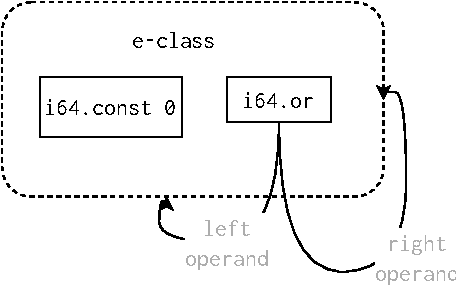
\includegraphics[width=0.7\linewidth]{figures/egraph1.pdf}
    \caption{e-graph for idempotent bitwise-or rewriting rule. Solid lines represent operand-operator relations, and dashed lines represent equivalent class inclusion. }
  \label{e-graph}
\end{figure}

% How to construct
For example, let us consider one program with a single instruction that returns an integer constant, \texttt{i64.const 0}. Let us also assume a single rewriting rule, \texttt{(x,\ x\ i64.or\ x, x instanceof i64)}. 
In this example, the program's control flow graph contains just one node, representing the unique instruction.
The rewriting rule represents the equivalence for performing an \texttt{or} operation with two equal operands.
\autoref{e-graph} displays the final e-graph data structure constructed out of this single program and rewriting rule. 
We start by adding the unique program instruction \texttt{i64.const 0} as an en e-node (depicted by the leftmost solid rectangle node in the figure). 
Next, we generate e-nodes from the rewriting rule (the rightmost solid rectangle) by introducing a new e-node, \texttt{i64.or}, and creating edges to the \texttt{x} e-node.
Following this, we establish equivalence. 
The rewriting rule combines the two e-nodes into a single e-class (indicated by the dashed rectangle node in the figure). 
As a result, we update the edges to point to the \texttt{x} symbol e-class.

%\todo{explain what "equality saturation" means in this context. do we use equality saturation for diversification? I'm not sure}
%Since there are no more rewriting rules to apply, we reach equality saturation, signifying that the graph can no longer change. Therefore, we have successfully constructed the e-graph.

\paragraph{e-graph Traversal Algorithm}
\label{alg}
% General use of case
While e-graphs possess numerous significant properties, we focus on what we believe is the most crucial for the purpose of diversification. We articulate this key attribute as an invariant in the text that follows.

\begin{tcolorbox}[boxrule=1pt,arc=.3em,boxsep=-1.3mm]
Any path traversal through the e-graph results in a semantically equivalent expression
\end{tcolorbox}

%\todo{which invariant? why does it matter?}
The invariant is exemplified in \autoref{e-graph}, where an infinite concatenation of "or" operations can be constructed. 
In this work, we take advantage of this invariant to generate mutated variants of an original program. 
The e-graph can be traversed randomly, selecting an e-node within each e-class that we visit, producing a random-but-equivalent expression. 
%We can extract an infinite number of semantically equivalent expressions from the e-graph, as shown in previous research \cite{10.1145/3571207, 10.1145/3434304}.

%It selects a random instruction within the binary functions and applies one or more of the 125 rewrite rules.
%Finally, it re-encodes the WebAssembly module with the new, rewritten expression to produce a binary variant. 


% - SMT and egraphs are complete different things. Therefore, we need to evaluate the soundness of the egraphs generated programs modulo Input => CROW
 
% - wasm-mutate only applies egraphs if the CFG of the peephole is complete/deterministic.


\algnewcommand\algorithmicforeach{\textbf{for each}}
\algdef{S}[FOR]{ForEach}[1]{\algorithmicforeach\ #1\ \algorithmicdo}
\begin{algorithm}
    \footnotesize
	\begin{algorithmic}[1]
	%	\Procedure{MyProcedure}{}
        \Procedure{traverse}{$egraph$, $eclass$, $depth$}
        % Input:
        %\Comment{Input: e-graph, max-depth}
        % Output:
        %\Comment{Output:y}
        \If{depth = 0}
          \State  \Return \textbf{smallest\_tree\_from}(egraph,\ eclass)
        \Else
            \State $nodes \gets egraph[eclass]$
            \State $node \gets random\_choice(nodes)$
            \State $expr \gets (node, operands=[])$
            \ForEach {$child \in node.children $}
                \State $subexpr \gets \textbf{TRAVERSE}(egraph,\ child,\ depth - 1)$
                \State $expr.operands \gets expr.operands \cup\ \{subexpr\}$
            \EndFor
            \State \Return $expr$
        \EndIf
        \EndProcedure
	\end{algorithmic} 
	\caption{e-graph traversal algorithm.} 
	\label{peephole:mutator}
\end{algorithm}

%\todo{can we make a strong claim here? does everybody maximize simplification with equality saturation? are we the first to do random path in e-grahs?}
We propose an algorithm to randomly traverse an e-graph and generate  semantically equivalent program variants.
The e-graph traversal is summarized in Algorithm \autoref{peephole:mutator}. 
To the best of our knowledge, \tool, is the first practical implementation of the random e-graph traversal algorithm.
It receives an e-graph, an e-class node (initially the root's e-class), and the maximum depth of expression to extract. The depth parameter ensures that the algorithm is not stuck in an infinite recursion. We select a random e-node from the e-class (lines 5 and 6), and the process recursively continues with the children of the selected e-node (line 8) with a decreasing depth. As soon as the depth becomes zero, the algorithm returns the smallest expression out of the current e-class (line 3). The subexpressions are composed together (line 10) for each child, and then the entire expression is returned (line 11). 

\paragraph{Example of a random e-graph traversal}
Let's demonstrate how the proposed traversal algorithm can generate program variants with an example. 
We will illustrate Algorithm \ref{peephole:mutator} using a maximum depth of 1. 
\autoref{example:peeporig} presents a hypothetical original Wasm binary to mutate. 
In this example, the developer has established two rewriting rules: \texttt{(x, x i32.or x, x instanceof i32)} and \texttt{(x, x i32.add 0, x instanceof i32)}. The first rewriting rule represents the equivalence of performing an \texttt{or} operation with two equal operands, while the second rule signifies the equivalence of adding 0 to any numeric value.
By employing the code and the rewriting rules, we can construct the e-graph depicted in \autoref{e-graph3}. The figure demonstrates the operator-operand relationship using arrows between the corresponding nodes.



\lstdefinestyle{watcode}{
  numbers=none,
  stepnumber=1,
  numbersep=10pt,
  tabsize=4,
  showspaces=false,
  breaklines=true, 
  showstringspaces=false,
    moredelim=**[is][{\btHL[fill=weborange!40]}]{`}{`},
    moredelim=**[is][{\btHL[fill=celadon!40]}]{!}{!}
}


   \begin{minipage}[b]{\linewidth}
    \lstset{
        language=WAT,
                        style=watcode,
        basicstyle=\footnotesize\ttfamily,
                        columns=fullflexible,
                        breaklines=true}
        
        \begin{lstlisting}[label=example:peeporig,caption={Wasm function.},frame=b, captionpos=b]{Name}
(module
    (type (;0;) (func (param i32 f32) (result i64)))
    (func (;0;) (type 0) (param i32 f32) (result i64)
        i64.const 1)
)
        \end{lstlisting}
\end{minipage}


\begin{minipage}[b]{\linewidth}
    \lstset{
        language=WAT,
                        style=watcode,
        basicstyle=\footnotesize\ttfamily,
                        columns=fullflexible,
                        breaklines=true}
        
        \begin{lstlisting}[label=example:peepapplied,caption={Random peephole mutation using egraph traversal for \autoref{example:peeporig} over e-graph \autoref{e-graph3}. The textual format is folded for better understanding.},frame=b, captionpos=b]{Name}
(module
    (type (;0;) (func (param i32 f32) (result i64)))
    (func (;0;) (type 0) (param i32 f32) (result i64)
        !(i64.or (!
            !(i64.add (!
                !i64.const 0!
                !i64.const 1!
            !))!
            !i64.const 1!
        !))!
    )
        \end{lstlisting}
\end{minipage}



\begin{figure}
    \centering
    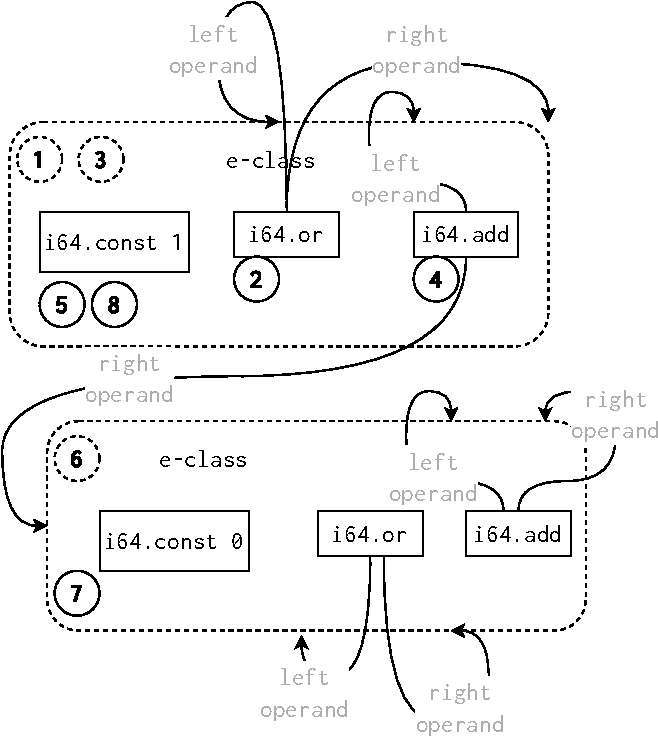
\includegraphics[width=0.75\linewidth]{figures/egraph3.pdf}
    \caption{e-graph built starting in the first instruction of \autoref{example:peeporig}. }
  \label{e-graph3}
\end{figure}


In \autoref{e-graph3}, we annotate the various steps of Algorithm \ref{peephole:mutator} 
for the scenario  described above. Algorithm \ref{peephole:mutator} begins at the e-class containing the single instruction \texttt{i64.const 1} from \autoref{example:peeporig}. 
It then selects an equivalent node in the e-class (2), in this case, the \texttt{i64.or} node, resulting in:
{\texttt{expr = i64.or l r}}.
The traversal proceeds with the left operand of the selected node (3), choosing the \texttt{i64.add} node within the e-class: 
{\texttt{expr = i64.or (i64.add l r)} \texttt{r}}.
The left operand of the \texttt{i64.add} node is the original node (5): 
{\texttt{expr = i64.or (i64.add i64.const 1 r)} \texttt{r}}.
The right operand of the \texttt{i64.add} node belongs to another e-class, where the node \texttt{i64.const 0} is selected (6)(7):
{\texttt{expr = i64.or (i64.add i64.const 1 i64.const 0)} \texttt{r}}.
In the final step (8), the right operand of the \texttt{i64.or} is selected, corresponding to the initial instruction e-node, returning:
{\texttt{expr = i64.or (i64.add i64.const 1 i64.const 0)\ i64.const 1}}
The traversal result applied to the original Wasm code can observed in \autoref{example:peepapplied}. 

\subsection{Implementation}

\tool is implemented in Rust, comprising approximately 10767 lines of Rust code. 
We leverage the capabilities of the wasm-tools project of the bytecodealliance for parsing and transforming WebAssembly binary code. 
Specifically, we utilize the wasmparser and wasm-encoder modules for parsing and encoding Wasm binaries, respectively.
The combination of wasmparser and wasm-encoder enables \tool to rewrite Wasm binaries. 
%All operations are done lazily: only the necessary sections of the binary are parsed and rewritten during the transformation of the input Wasm by \tool.
The implementation of \tool can be found at \repourl.

%\todo{J: Should we talk about determinism in the transformations?}



%Although the construction of the e-graph itself can be expensive, we can reuse the e-graph many times after construction, amortizing the construction costs. 
%We can also speed up construction by limiting the number of rewrites applied to the e-graph. 


%\textbf{Add global}
%\todo{Move this to special operators in the peephole mutator}
%
\lstdefinestyle{watcode}{
  numbers=none,
  stepnumber=1,
  numbersep=10pt,
  tabsize=4,
  showspaces=false,
  breaklines=true, 
  showstringspaces=false,
    moredelim=**[is][{\btHL[fill=black!10]}]{`}{`},
    moredelim=**[is][{\btHL[fill=celadon!40]}]{!}{!}
}

{\captionsetup{width=0.45\linewidth}
\noindent\begin{minipage}[b]{0.45\linewidth}
    \lstset{
        language=WAT,
        style=watcode,
        basicstyle=\footnotesize\ttfamily,
        columns=fullflexible,
        breaklines=true}
        \begin{lstlisting}[label=example:block1,caption={Add global.},frame=b, captionpos=b]{Name}
...
!+ !
...
        \end{lstlisting}
        %\vspace{0.2cm}
   \end{minipage}\hfill%
\noindent\begin{minipage}[b]{0.45\linewidth}
    \lstset{
        language=WAT,
                        style=watcode,
        basicstyle=\footnotesize\ttfamily,
                        columns=fullflexible,
                        breaklines=true}
        
        \begin{lstlisting}[label=example:block2,caption={Remove global.},frame=b, captionpos=b]{Name}
...
`- `
...   
        \end{lstlisting}
\end{minipage}
}


%\subsection{Properties}

%- Ergodicity (validates malware evasion paper)

%- Faster (compare to other rewriting tools, CROW)

%- Taxonomy, easy to measure and control the rewriting space. Define properties and metrics, e.g. size of the rewriting.
\vspace{-2mm}
\section {Evaluation}
\label{eval}

In this section, we outline our methodology for evaluating \tool.
Initially, we introduce our research questions and the corpus of programs that we utilize for the assessment of \tool.
Next, we elaborate on the methodology for each research question.
Our data and experimenting pipeline are publicly available at \dataurl.

%\subsection{Research Questions}

\newcommand\rqstatic{To what extent are the program variants generated by \tool statically different from the original programs?\xspace}

\newcommand\rqdynamic{To what extent are the program variants generated by \tool dynamically different from the original programs?\xspace}

\newcommand\rqdefensive{To what extent does \tool prevent side-channel attacks on \Wasm programs?\xspace}


\newcommand\rqperformance{To what extent does \tool affects the performance of \Wasm program variants?\xspace}


\newcommand\rqtesting{To what extent can \tool be used to perform differential testing of \Wasm tools?\xspace}

\newcommand{\nProgramsRosetta}{303\xspace}


\newcommand{\DTWStatic}{\ensuremath{\mathit{dt\_static}\xspace}}
\newcommand{\DTWDynamic}{\ensuremath{\mathit{dt\_dy}\xspace}}

\begin{enumerate}[label=RQ\arabic*:, ref=RQ\arabic*]
    % From CROW %%%%%%%%%%%%%%%%%%%%%%%%%%%%%%%%%%%%%%%%%%%%%%%%%%%%%%%%%%%%%%%%%%%
     \item \label{rq:static} \textbf{\rqstatic}
        We  check whether the \wasm binary variants produced by \tool are different from the original \wasm binary. Then, we assess whether the x86 machine code produced by wasmtime engine is also different.
    
    \item \label{rq:dynamic}\textbf{\rqdynamic} 
        It is known that not all diversified programs produce distinguishable executions \cite{crane2015thwarting}. 
        We check for the presence of different behaviors by collecting execution traces, characterizing the behavior of a \wasm program by its machine code memory and instruction traces.
    %%%%%%%%%%%%%%%%%%%%%%%%%%%%%%%%%%%%%%%%%%%%%%%%%%%%%%%%%%%%%%%%%%%%%%%%%%%%%%%
        
    \item \label{rq:defensive}\textbf{\rqdefensive} 
     \label{rq:performance} Diversification being an option to prevent security issues,  we assess the impact of \tool in preventing one class of attacks: cache attacks (Spectre).
        
\end{enumerate}

\subsection{Corpora}
\label{sec:corpus}


\begin{table}
\renewcommand\arraystretch{1.1}
\begin{adjustbox}{width=\linewidth,totalheight=\textheight, keepaspectratio}
{
\color{blue}
    \begin{tabular}{p{1.5cm} | l | l | r | r | p{2cm}  }
        \hline
        Source & Program & RQ & \#F & \# Ins. & Attack  \\
        \hline \hline
        CROW \cite{arteaga2020crow} & 303 & \ref{rq:static}, \ref{rq:dynamic} & 7-103 & 170-36,023 & N/A  \\
        \hline

        wasmbench \cite{hilbig2021empirical} & 134 & \ref{rq:performance} & 1-8,375 & 11-1,162,469 & N/A \\
        
        \hline

        Swivel \cite{Swivel} & btb\_breakout & \ref{rq:defensive} & 16 & 743 & Spectre branch target buffer (btb)  \\
        \hline
        Swivel \cite{Swivel}  & btb\_leakage & \ref{rq:defensive} & 16 & 297 & Spectre branch target buffer(btb)  \\
        \hline
        Safeside \cite{Swivel, safeside}  & ret2spec & \ref{rq:defensive} & 2,977 & 378,894 & Spectre Return Stack Buffer (rsb)  \\
        \hline
        Safeside  \cite{Swivel, safeside} & pht & \ref{rq:defensive} & 2,978 & 379,058 & Spectre Pattern History Table (pht)  \\

        

%\end{adjustbox}
    \end{tabular}
}
\end{adjustbox}
    
    \caption{The dataset we use to evaluate \tool. Each row in the table corresponds to programs, with the columns providing: where the program is sourced from, the number of programs, research question addressed, function count, the total number of instructions found in the original \wasm program and the type of attack that the original program was subjected to.}
    \label{tab:corpus}
\end{table}


We answer our research questions with a corpus of 307 programs (303 + 4).
These programs are summarized in \autoref{tab:corpus}.
Each row in the table corresponds to the used programs, with the columns providing: where the program is sourced from, the number of programs, research question addressed, function count, the total number of instructions found in the original \wasm program and the type of attack that the original program was subjected to.

We answer \ref{rq:static} and \ref{rq:dynamic} with corpus of programs from Cabrera \etal \cite{arteaga2020crow}, it is shown in the first row of \autoref{tab:corpus}.
The corpus contains \nProgramsRosetta.
The corpus contains programs for a range of tasks, from simple ones, such as sorting, to complex algorithms like a compiler lexer. 
The number of functions for each program ranges from 7 to 103 and, the number of total instructions ranges from 170 to 36023.
All programs in corpus: 
1) do not require input from user, \ie do not  functions like \texttt{scanf}, 2) terminate, 3) are deterministic, \ie given the same input, provide the same output and 4) compile to \wasm using \texttt{wasi-clang} to compile them.

We answer \ref{rq:defensive} with four \Wasm programs and three Spectre attack scenarios, from the Swivel project \cite{Swivel}. 
These programs are summarized in the final four rows of our corpus table.
The first two programs are manually crafted and contain 16 functions, with instruction counts of 743 and 297, respectively. These binaries are specifically designed to perform the Spectre branch target attack.
The third and fourth programs, documented in rows four and five, comefrom the Safeside project \cite{safeside}. 
Unlike the first two, these binaries are significantly larger, each containing nearly 3000 functions and more than 300000 instructions. 
They are utilized for conducting the Spectre Return Stack (RSB) and Spectre Pattern History (PHT) attacks \todo{add reference}.

There is a notable difference in the number of functions and instructions between the first pair of Swivel binaries and the latter pair. 
This disparity can be attributed to the varying compilation processes applied to these \Wasm binaries. 
% The first two were manually tailored to streamline the attack processes, whereas the other two programs were directly compiled from Safeside \cite{safeside}.
The three attack scenarios are described in details in \autoref{protocol:rq3}.

%% FROM CROW RQ1
\subsection{Protocol for RQ1}
\label{protocol:rq1}

\begin{figure}
    \centering
    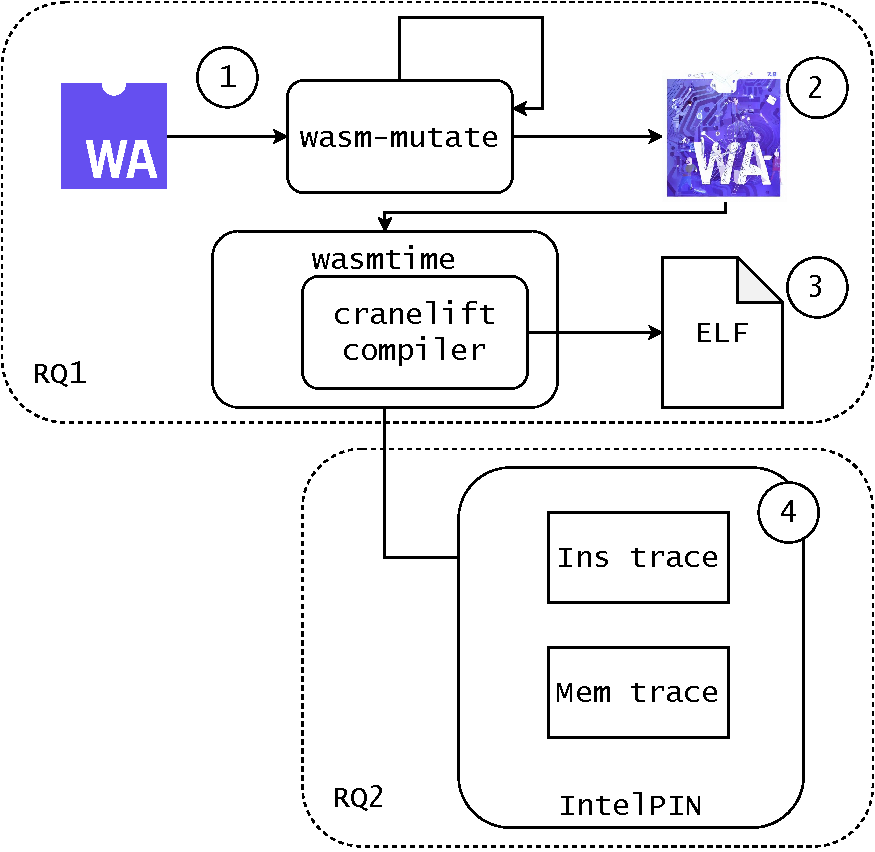
\includegraphics[width=0.8\linewidth]{figures/protocol.pdf}
    \caption{Protocol to answer \ref{rq:static} and \ref{rq:dynamic}}
  \label{protocol}
\end{figure}


With \ref{rq:static},
we assess the ability of \tool to generate \Wasm binaries that are different from the original program, including after their compilation to x86 machine code.
In \autoref{protocol} we show the steps we follow to answer \ref{rq:static}.
We run \tool on our corpus of \nProgramsRosetta{} original C programs (step \step{1} in figure). 
To generate the variants:
% Select wih replacement algo
1) we start with one original and pass it to \tool to generate a variant;  
2) the variant and the original program form a population of programs; 
3) we randomly select a program from this population and pass it to \tool to generate a variant, which we add to the population; 
4) we then restart the process in the previous step. to stack more mutations 
This procedure is carried out for a duration of 1 hour.
The final outcome (step \step{2} in figure) is a population with a number of stacked transformations, all starting from an original \wasm program.
We then count the number of unique variants in the population.
We compute the sha256 hash of each variant bytestream in order and define the population size metric as: 


\begin{metric}{Population\_size(P):}\label{metric:pop}
Given an original \wasm program P, a generated corpus of \wasm programs $V=\{v_1, v_2, ..., v_N\}$ where $v_i$ is a variant of P, the population size is defined as:
$$
    | set(\{ sha256(v_1), ... sha256(v_N) \})|\text{ }\forall v_i \in V 
$$
\end{metric}


Since \wasm binaries may be further transformed into machine code before they execute, we also check that this additional transformations preserve the difference introduces by \tool in the \wasm binary. 
We use the wasmtime JIT compiler, cranelift, with all available optimizations, to generate the x86 binaries for each \wasm program and its variants  (step \step{3} in figure). 
Then, we calculate the number of unique variants machine code representation for wasmtime.
Counting the number of unique machine code, we compute the diversification preservation ratio: \\

\begin{metric}{Ratio of preserved variants:}\label{metric:preservation}
    Given an original \wasm program P and its population size as defined in \autoref{metric:pop} and the JIT compiler C, we defined the ratio of preserved variants as:
    $$
        \frac{ | set(\{ sha256(C(v_1)), ... sha256(C(v_N)) \})|}{ \text{Population\_size (P)}} \text{ }\forall v_i \in V 
    $$

    
\end{metric}

If \\ $sha256(P_1)$ $\neq$ $sha256(P_2)$ and $sha256(C(P_1))$) $\neq$ $sha256(C(P_2))$, this means that  both programs are still different after being compiled to machine code, and this means that the cranelift compiler has not removed the transformations made by \tool.  



%% FROM CROW RQ2
\subsection{Protocol for RQ2}
\newcommand{\samples}{100\xspace}

For \ref{rq:dynamic}, we compare  the executions of an original program and its variants for a given input.
This process can be appreciated in the enclosed square of \autoref{protocol}, annotated with \ref{rq:dynamic}.
We execute the program using wasmtime, a standalone runtime for \Wasm. 
We chose wasmtime because of its widespread adoption, reflecting its high level of maturity.
For instancce, wasmtime, is the core of the Content Delivery Network of Fastly.
%\todo{one sentence to explain what wasmtime is and how notable it us}
In this experiment, we characterize the  execution of a \wasm binary according to its traces when running in wasmtime.

We first collect \wasm binaries for which wasmtime generates unique machine code, i.e., variants that are preserved (refer to \autoref{protocol:rq1}).
Then we execute a random sample of \samples \wasm variants for each original program.
For each execution of a \wasm program, we gather the instructions and memory traces utilizing IntelPIN \cite{luk2005pin, 10.1145/3478520} (step \step{4} in the figure).
To only collect the traces of the Wasm execution with a wasmtime engine, we pause and resume the collection as the execution leaves and re-enters the Wasm code, respectively.
We implement this filtering with the built-in hooks of wasmtime.
In addition, we disable ASLR on the machine where the variants are executed.
This latter action ensures that the placement of the instructions in memory is deterministic.
For the memory trace , we take those events that originate from an instruction of a Wasm code and end up into the linear memory region of the same Wasm binary.
Examples of the traces we collect can be seen in \autoref{example:trace1} and \autoref{example:trace2} for memory and instruction traces, respectively.


\lstdefinestyle{watcode}{
  numbers=none,
  stepnumber=1,
  numbersep=10pt,
  tabsize=4,
  showspaces=false,
  breaklines=true, 
  showstringspaces=false,
    moredelim=**[is][{\btHL[fill=weborange!40]}]{`}{`},
    moredelim=**[is][{\btHL[fill=celadon!40]}]{!}{!}
}


   \begin{minipage}[b]{\linewidth}
    \lstset{
        language=TRACE,
                        style=watcode,
        basicstyle=\footnotesize\ttfamily,
                        columns=fullflexible,
                        breaklines=true}
        
        \begin{lstlisting}[label=example:trace1,caption={Memory trace  with two events out of IntelPIN for the execution of a \wasm program with wasmtime. Trace events record: the type of the operation, read or write, the memory address, the number of bytes affected and the value read or written.},frame=b, captionpos=b]{Name}
[Writ]                                                           0x555555ed1570 size=4 value=0x10dd0
[Read]                                                           0x555555ed1570 size=4 value=0x10dd0                      \end{lstlisting}
\end{minipage}


\begin{minipage}[b]{\linewidth}
    \lstset{
        language=TRACE,
                        style=watcode,
        basicstyle=\footnotesize\ttfamily,
                        columns=fullflexible,
                        breaklines=true}
        
        \begin{lstlisting}[label=example:trace2,caption={Instructions trace with two events out of IntelPIN for the execution of a \wasm program with wasmtime. Each event records the corresponding machine code that executes.},frame=b, captionpos=b]{Name}
[I]          mov rdx, qword ptr [r14+0x100]           
[I]          mov dword ptr [rdx+0xe64], ecx          
    \end{lstlisting}
\end{minipage}


In the text below, we outline the metric applied to the traces, which is used to assess the variability in the behavior of different variants.

\begin{metric}{Ratio of different traces:}\label{metric:mem:sha}
Given an original \wasm program P, a generated corpus of \wasm variants $V=\{P,v_1, v_2, .., v_N\}$ and a collection of traces of type $E\in \{Mem, Inst\}$, $T=\{P_E, v_1E, v_2E, ...v_3E\}$ out of executing each variant, the ratio of different traces of an event type E is defined as:
$$
    \frac{| set(\{ sha256({P_E}),..., sha256(v_NE) \})|}{| \{ sha256(P_E),..., sha256(v_NE) \}|}\text{ } \forall v_i \in T
$$

\end{metric}

Notice that the previously defined metric is instantiated twice, for instructions and memory type of events.
A Ratio of 1 means that all \wasm variants produce different traces, a ratio of 0 means that all variants produce exactly the same traces, so the higher the better.

%\todo{this is not for RQ2. and we do not have RQ about performance anymore, what can we do? J: Either we drop it or we explain why execution time is important for side-channels. But since we have a performance evaluation in the evasion paper, I vote for droping.}
%We also calculate the execution times for the preserved variants and their corresponding original programs.
%This can be appreciated in step \step{5} of the figure.
%For each compiled population we randomly select \samples binaries including the original.
%We then execute each binary 100 times to collect a distribution for which we measure its median value.


\subsection{Protocol for RQ3}
\label{protocol:rq3}

\newcommand{\poct}{\emph{Cache timing POC}\xspace}
\newcommand{\pocd}{\emph{Differential computing POC}\xspace}
\newcommand{\pocp}{\emph{Port contention POC}\xspace}

To answer \ref{rq:defensive}, we apply \tool to the same security \wasm programs used by Narayan et al. to evaluated Swivel's ability at protecting \wasm programs against side-channel attacks \cite{Swivel}. 
The four cache timing side-channel attacks are presented in detail in \autoref{sec:corpus}. 
The specific binary and its corresponding attack can be appreciated in \autoref{tab:corpus}.
We evaluate to what extent \tool can prevent such attacks.
In the following text, we describe the attacks we replicate and evaluate in order of answering \ref{rq:defensive}.

%\todo{move the description of the four binaries in  \autoref{sec:corpus} and here add a short description of the intuition why \tool could be useful to prevent the attacks}

% Describing the Speculative execution  POC
%\todo{what does "successfully navigated around the control flow integrity safeguards" mean?}
Narayan and colleagues successfully bypass the control flow integrity safeguards, using speculative code execution as detailed in \cite{Spectre}. 
Thus, we use the same three Spectre attacks from Swivel:
1) The Spectre Branch Target Buffer (btb) attack exploits the branch target buffer by predicting the target of an indirect jump, thereby rerouting speculative control flow to an arbitrary target.
2) The Spectre Pattern History Table (pht) takes advantage of the pattern history table to anticipate the direction of a conditional branch during the ongoing evaluation of a condition. 
3) The Spectre Return Stack Buffer (ret2spec) attack exploits the return stack buffer that stores the locations of recently executed call instructions to predict the target of \texttt{ret} instructions. 
Each attack methodology relies on the extraction of memory bytes from another hosted \wasm binary that executes in parallel.


For each of the four \wasm binaries introduced in \autoref{sec:corpus}, we generated a maximum of 1000 random stacked transformations utilizing 100 distinct seeds. 
This resulted in a total of 100,000 variants for each original \wasm binary.
We then assess the success rate of attacks across these variants by measuring the bandwidth of the exfiltrated data, that is: the rate of correctly leaked bytes per unit of time. 
We then count the correctly exfiltrated bytes and divided them by the variant program's execution time. 

Notice that, the bandwidth metric captures not only whether the attacks are successful or not, but also the degree to which the data exfiltration is hindered.
For instance, a variant that continues to exfiltrate secret data but does so over an impractical duration would be deemed as having been hardened. 
For this, we state the bandwidth metric in the following definition :

\begin{metric}{Bandwidth:}\label{metric:ber}
Given data $D=\{b_0, b1, ..., b_C\}$ being exfiltrated in time $T$ and $K = {k_1, k_2, ..., k_N}$ the collection of correct data bytes, the bandwidth metric is defined as:
$$
    \frac{|b_i\text{ such that } b_i \in K|}{T}
$$
\end{metric}







\section{Experimental Results}
\label{results}

\subsection{\rqstatic}
\label{rq:static:results}

\newcommand{\preserved}{72\%\xspace}

% Recap
To address \ref{rq:static}, we utilize \tool to process the original 303 programs from \cite{arteaga2020crow}. 
\tool is set to generate variants with a timeout of one hour for each individual program. 
Following this, we assess the sizes of their variant populations as well as their corresponding preservation ratio (Refer to \autoref{metric:pop} and \autoref{metric:preservation} for more details).

\begin{figure}
    \centering
    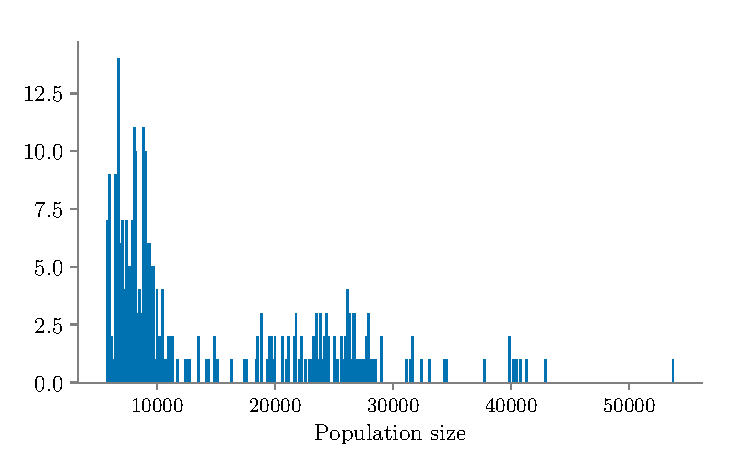
\includegraphics[width=\linewidth]{plots/rq1/population.pdf}
    \caption{Number of unique \wasm programs generated by \tool in 1 hour out of each program of the CROW's corpus.}
  \label{rq1:plot:population}
\end{figure}


% Explain figure 4 and how wm outperform CROW in number of variants
In \autoref{rq1:plot:population}, we show the population size generated out of \tool. 
Each X point corresponds to a particular program, arranged in descending order based on population size. 
The Y-axis denotes the population size. 

% General numbers
\tool successfully diversifies all 303 original programs, yielding a diversification rate of 100\%. 
Within an hour, \tool demonstrates its impressive efficiency and effectiveness by producing a median of 9500 unique variants for the 303 original programs. \todo{one sentence about max and min value}
There are several factors contributing to large population sizes. 

% More space to diversify
\tool can diversify functions within WASI-libc. 
Despite the relatively low function count in the original source code,  \tool creates thousands of distinct variants in the function of the incorporated libraries. 
This feature improves over methods that can only diversify the original source code processed through the LLVM compilation pipeline \todo{\cite{XXX}}. 

\todo{weak and vague paragraph; substantiate or remove?}
Furthermore, the usage of an e-graph to model semantically equivalent codes significantly enhances variant generation. 
As previously highlighted, an e-graph unlocks the possibility of generating an infinite number of variants, thereby creating a much larger space for diversity.


% Now why not all populations are not the same
We have observed a significant variation in the population size out of \tool between different programs, ranging by several thousand variants. 
For example, the largest population size observed is 53816, while the smallest is 5716.
This disparity is attributed to:
the non-deterministic nature of \tool and 2) the characteristics of the program. 
\tool mutates a randomly selected portion of a program. 
If the selected instruction is determined to be non-deterministic, despite the transformation being semantically equivalent, \tool discards the variant and moves on to another random transformation.
For instance, if the instruction targeted for mutation is a function call, \tool proceeds to the next one.
This process, in conjunction with the unique characteristics of each program, results in a varying population size. 
For example, an input binary with a high number of function calls would lead to a greater number of trials and errors, slowing down the generation of variants, thereby resulting in a smaller overall population size for 1 hour of \tool execution.

% Describing the preservation plot
As stated in \autoref{protocol:rq1}, we take into account \autoref{metric:preservation} by calculating the preservation ratio. 
\autoref{rq1:plot:preservation} presents the preservation ratio for the cranelift compiler. 
In the figure, each point denotes the preservation ratio for a population for one single original program.
The arrangement of the points in the X axis mirrors the order of the \wasm population sizes showed in \autoref{rq1:plot:population}. 
This plot elucidates that there is no correlation between population size and preservation ratio. 
In other words, a larger population size does not necessarily correspond to a higher preservation ratio.
%, arranged in descending order. 


\begin{figure}
    \centering
    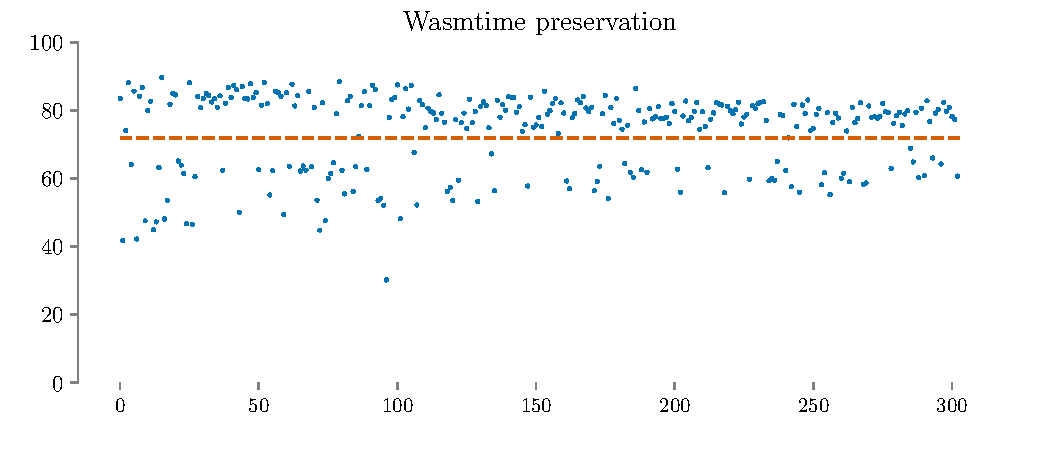
\includegraphics[width=\linewidth]{plots/rq1/preservation.pdf}
    \caption{Ratio of preserved variants.}
  \label{rq1:plot:preservation}
\end{figure}

% General numbers
Wwe observed a median preservation ratio of \preserved. 
The non-preserved transformations are explained as follows. 
Custom sections are disregarded by compilers.
Similarly, bloated code is another factor. 
\tool generates certain variants with unused types or functions, which are detected and eliminated by cranelift.


%%% too subtle, not actionable removing
%Interestingly, we've observed another noteworthy case.
%While cranelift can easily remove superfluous code inserted by \tool, they may be constrained by the quantity of resources they can allocate for optimizing machine code generation.  Consequently, some transformations, albeit "easy" to detect, might exceed this resources, and end up being retained in the compiled machine code.


% While preservation is not necesarilly good...conclude with this
\todo{Martin does not understand at all this paragraph: what's the take away}
While a lower preservation rate might not appear advantageous at first glance, our observations highlight that unpreserved variants can put certain compiler components under stress, components that remain dormant during the execution of the original binary. 
In essence, specific optimization implementations may remain idle if the corresponding code isn't included in the \wasm program set for compilation. 
Importantly, despite considering the smallest population size coupled with the lowest preservation percentage, the range of machine codes executed still encompasses thousands of variants, underscoring the effectiveness of diversification strategies.


%\begin{figure*}
%    \centering
%    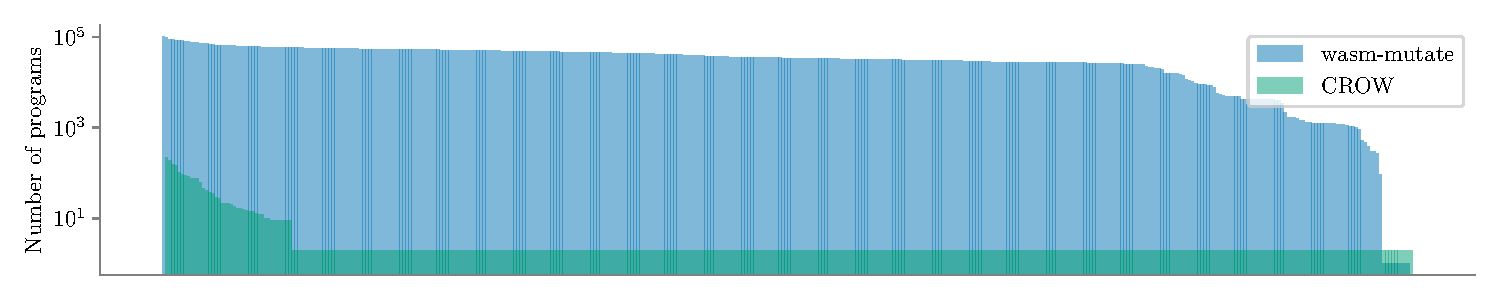
\includegraphics[width=0.9\linewidth]{plots/rq1/count.pdf}
%    \caption{TODO.}
%  \label{programs_count}
%\end{figure*}




\begin{tcolorbox}[boxrule=1pt,arc=.3em,boxsep=-1.3mm]
  \textbf{Answer to \ref{rq:static}}: \tool generates \wasm variants for the 303 programs, which are different from the original program. 
  Within a one-hour diversification budget, \tool synthesizes more than 9000 unique  variants per program on average. 
  \preserved of the variants remain different after machine-code compilation.
  \tool is good at producing a large number of \Wasm program variants.
\end{tcolorbox}


\subsection{\rqdynamic}

To answer \ref{rq:dynamic} we execute a random sample of variants with different machine code and their corresponding original programs with wasmtime.
We then collect execution times as well as, instructions and memory traces.
Finally, we calculate the number of different traces (refer to \autoref{metric:mem:sha}).

\begin{figure}
    \centering
    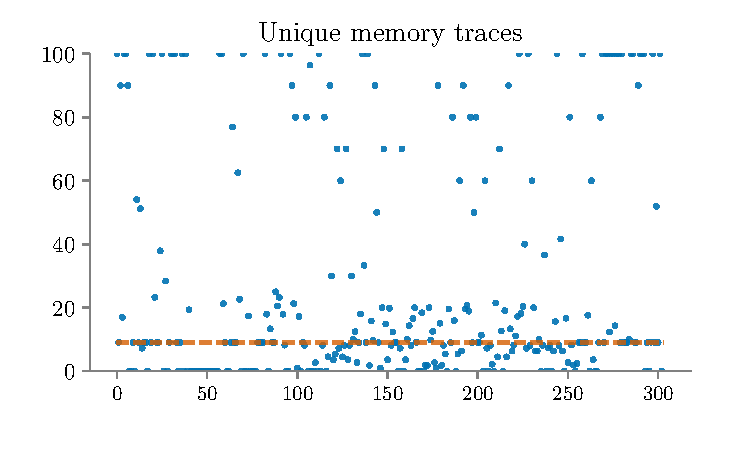
\includegraphics[width=\linewidth]{plots/rq2/memory.pdf}
    \caption{Ratio of memory trace differences. The higher the better. Dashed orange line represents the median ratio of unique memory traces for all programs and their variants.}
  \label{rq2:plot:mem}
\end{figure}

\begin{figure}
    \centering
    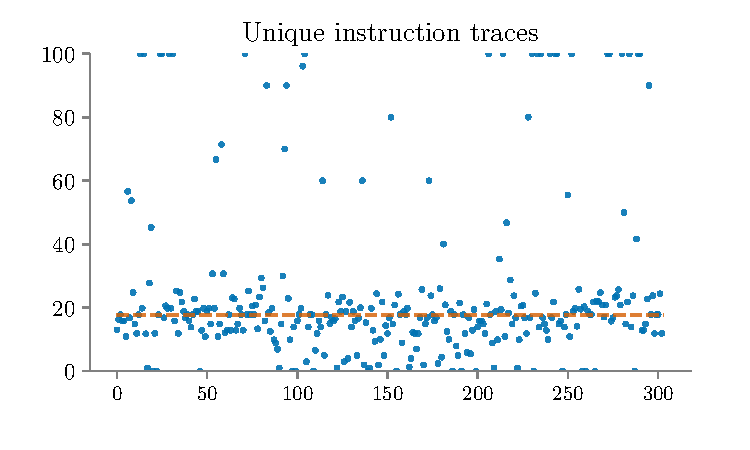
\includegraphics[width=\linewidth]{plots/rq2/instructions.pdf}
    \caption{Ratio of instruction trace differences. The higher the better. Dashed orange line represents the median ratio of unique instruction traces.}
  \label{rq2:plot:ins}
\end{figure}

% Plot 1 and 2 for different traces

\newcommand{\memratio}{9\%\xspace}
\newcommand{\insratio}{7\%\xspace}

In \autoref{rq2:plot:mem} and \autoref{rq2:plot:ins} we plot the uniqueness ratio for memory and instructions respectively.
Each X value represents an original program.
The blue dots represent the uniqueness ratio from 0 to 100.
For each compiled population we have observed that there is at least one variant that offer different execution traces, either for memory or machine code instructions.
The median number of different traces is \memratio and \insratio for memory and machine code instructions respectively.
We observe no correlation between the unique population size and the uniqueness of memory nor instruction traces (the X axis sorts programs by original size).

% Source of different mem traces
\todo{excellent paragraph}
We have identified four primary factors explaining why execution traces differs.
First, modifications to the binary layout inevitably alter both instruction traces and memory accesses within the program's stack. 
Specifically, \tool generates variants that modify the return addresses of functions, which consequently leads to differences in execution traces, including memory accesses.
Second, one of our rewriting rules incorporates artificial global values into \wasm binaries. 
Since these global variables are inherently manipulated via the stack, and given that the stack is located within linear memory, their access inevitably generates divergent memory traces.
Third, \tool injects 'phantom' instructions which do not aim to modify the outcome of a transformed function during execution. 
These intermediate calculations trigger the spill/reload component of cranelift, varying spill and reload operations. 
In the context of limited physical resources, these operations temporarily store values in memory for later retrieval and use, thus creating unique memory traces.
Finally, certain rewriting rules implemented by \tool replicate fragments of code, e.g., performing commutative operations. 
These code segments may contain memory accesses, and while neither the memory addresses nor their values change, the frequency of these operations does.
Overall, these findings influence the diversity of execution traces among the executed variants. 


% Source of identical traces

%\begin{figure}
%    \centering
%    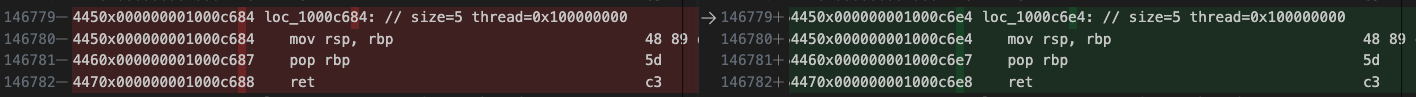
\includegraphics[width=\linewidth]{images/shifted_instructions.png}
%\end{figure}



% Different instruction count and memory count
\todo{"instruction count" and "memory count" never explained in the methodology for RQ. this paragraph mixes "instruction count", "memory count" and "execution times", which makes it hard to understand. one easy fix is to not talk about all of them, for instance just of execution times}
Moreover, we have observed considerable variation in the count of instructions, inclusive of memory accesses, among the distinct variants generated by \tool.
Intriguingly, a significant portion of these variants have a lower instruction count than their original program. 
This implies that \tool has the capability to enhance optimization of the original program, surpassing the innate optimizations employed by the wasmtime compiler. 
As a result, \tool is able to produce variants that outperform the original program in terms of execution time.
To provide a clearer depiction of this occurrence, we offer a graphical representation of the median execution times for all variants along with their original programs in \autoref{rq2:plot:execution_times}. 
Each individual data point on the plot signifies the median execution time for a specific variant, whereas the orange markers represent the median execution time for the original program.
Moreover, each vertical bar within the plot designates a distinct program population. 
Notice that relative comparisons between different vertical groups do not provide meaningful insights, as each group represents a distinct population of variants.

\begin{figure}
    \centering
    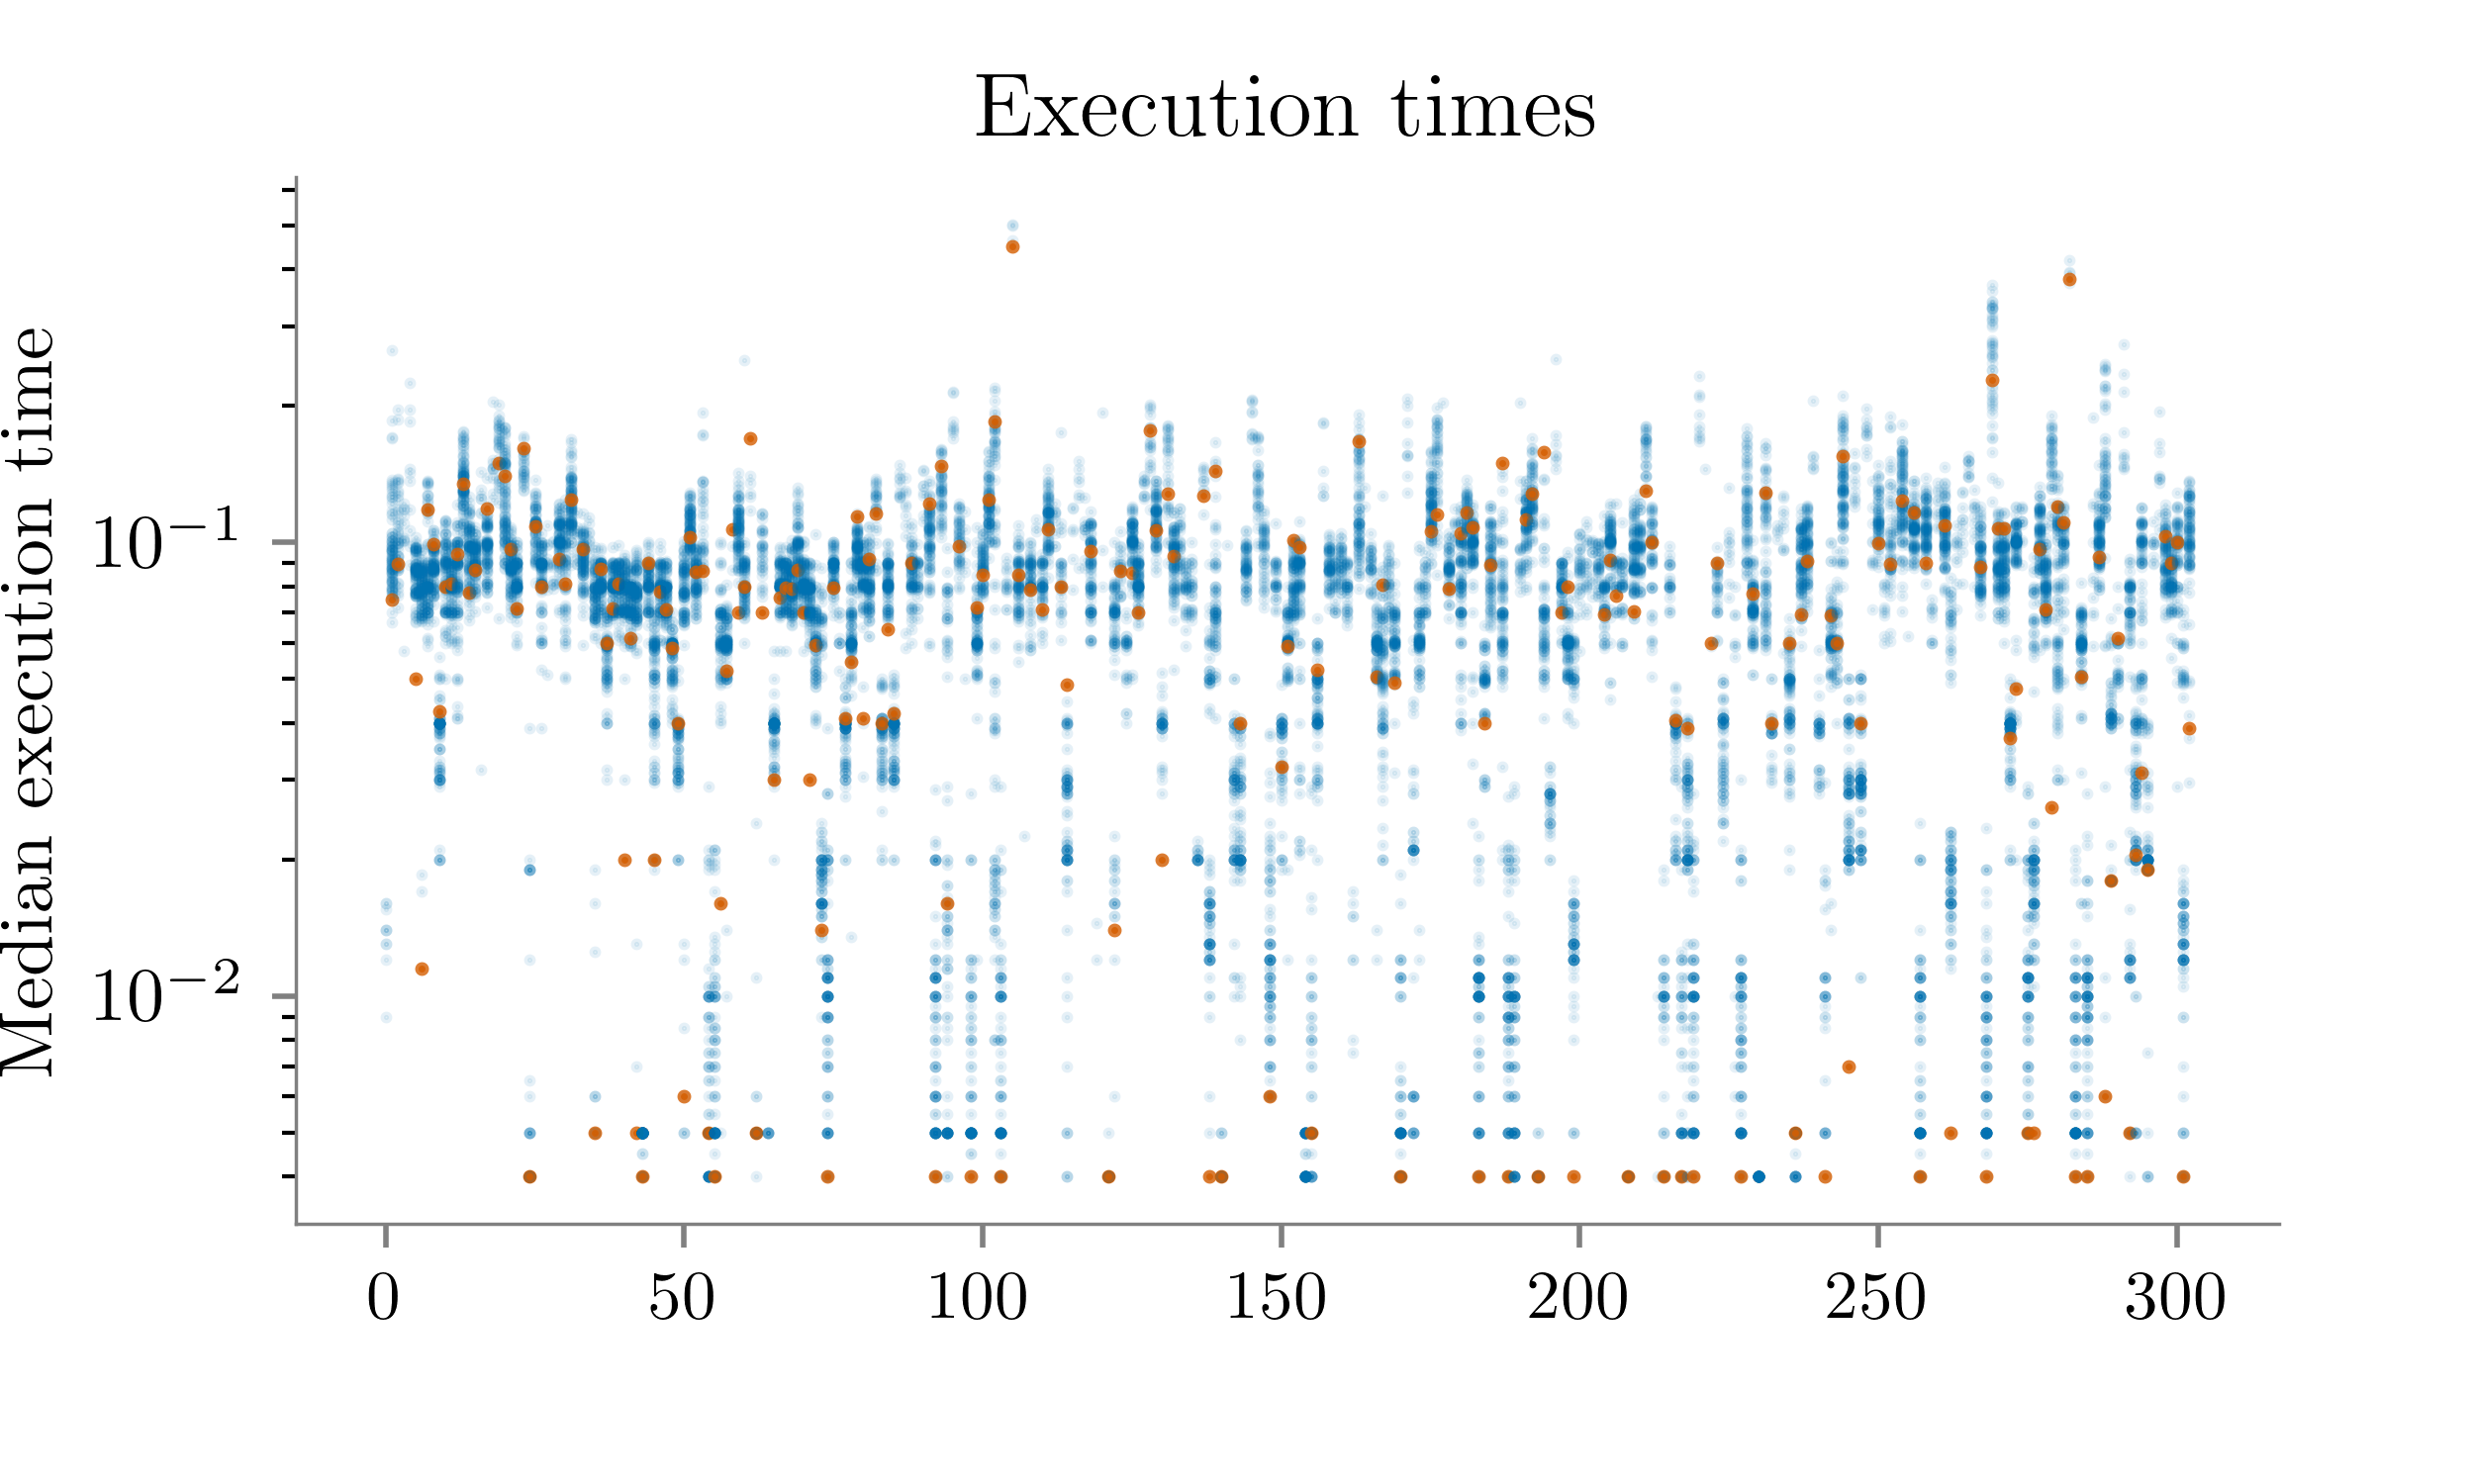
\includegraphics[width=\linewidth]{plots/rq2/times.png}
    \caption{Execution times or the original program and 100 variants of their population. In orange the median execution time of the original program. In blue the median execution time of 1 variant. Vertical groups represent different populations.}
  \label{rq2:plot:execution_times}
\end{figure}



% Words on the workload of each program
\todo{different input = different trace is a truism, which might be what would be understood by the reader. I see where you want to go but it's too subtle, and it highlights the weakness of the dataset (no input), so I would remove }
Notice that, each program and its variants are executed with their initial input.
In practice, the traces we collect are generated from instantiating the \wasm binary and then executing its main function. 
For most programs in the CROW suite, their main function carries out a specific algorithm (for instance, \emph{base64 encoding}) using a simple, single-input model. 
This approach helps to collect execution traces without crafting programs input.
Yet, it potentially reduce the uniqueness of the traces collected. 
For instance, sections of the program subject to conditional execution might not be activated, not necessarily due to their 'dead-code' status, but rather due to the limited variety of inputs. 
However, even with this relatively modest input-testing approach, \tool still succeeds in providing more than one unique execution trace for each program and its variants population.
it is worth noting that the ratio of unique traces would likely increase given a broader input spectrum.

% Conclude with a history of X original, generates in median 9000 variants in 1 hour, after preservation in wasmtime this number goes to 4000, after our numbers...1000 offer different execution traces.
Reflecting on the findings from \ref{rq:static} regarding preservation, we notice that the number of generated variants displaying diverse runtime behaviors remains remarkable. 
Let us illustrate this with an example.
\tool generates a median of 9000 variants in only 1 hour, for the original programs described in the answer to \ref{rq:static}. 
Of these \wasm variants, around \preserved are preserved in wasmtime, resulting into an effective total of 6480 distinct machine code programs.
\todo{here we mix average number of total number, very confusing, rework and ping me back}
Considering our data in \ref{rq:dynamic}, hundreds (\memratio$\times$6480) of these programs present unique execution traces, either through differentiated memory accesses or the overall variation in executed instructions. 
Therefore, \tool effectively generates \wasm program variants that challenge all aspects of a \wasm binary's lifecycle within wasmtime: from the initial compilation into machine code to its ultimate execution. 
This showcases the profound influence of \tool on diversifying and stressing the runtime environment.

\todo{add a discussion subsection about the process of using wasm-mutate in paragraph: diversify, identify at testing time with some workload or input creator one variant that is dynamically different and use this one in production. add a re from there. that process might even be in the tech section rather than in the Dicussion section}

\begin{tcolorbox}[boxrule=1pt,arc=.3em,boxsep=-1.3mm]
  \textbf{Answer to \ref{rq:dynamic}}:   \tool crafts variants that showcase diverse instruction traces and distinct memory accesses. 
  In every case, there is at least one variant among the compiled population that does produce a different trace. 
  With a large enough population of \wasm variants, \tool guarantees unique execution traces for at least one of them. 
\end{tcolorbox}


\subsection{\rqdefensive}



\begin{figure*}
    \centering
    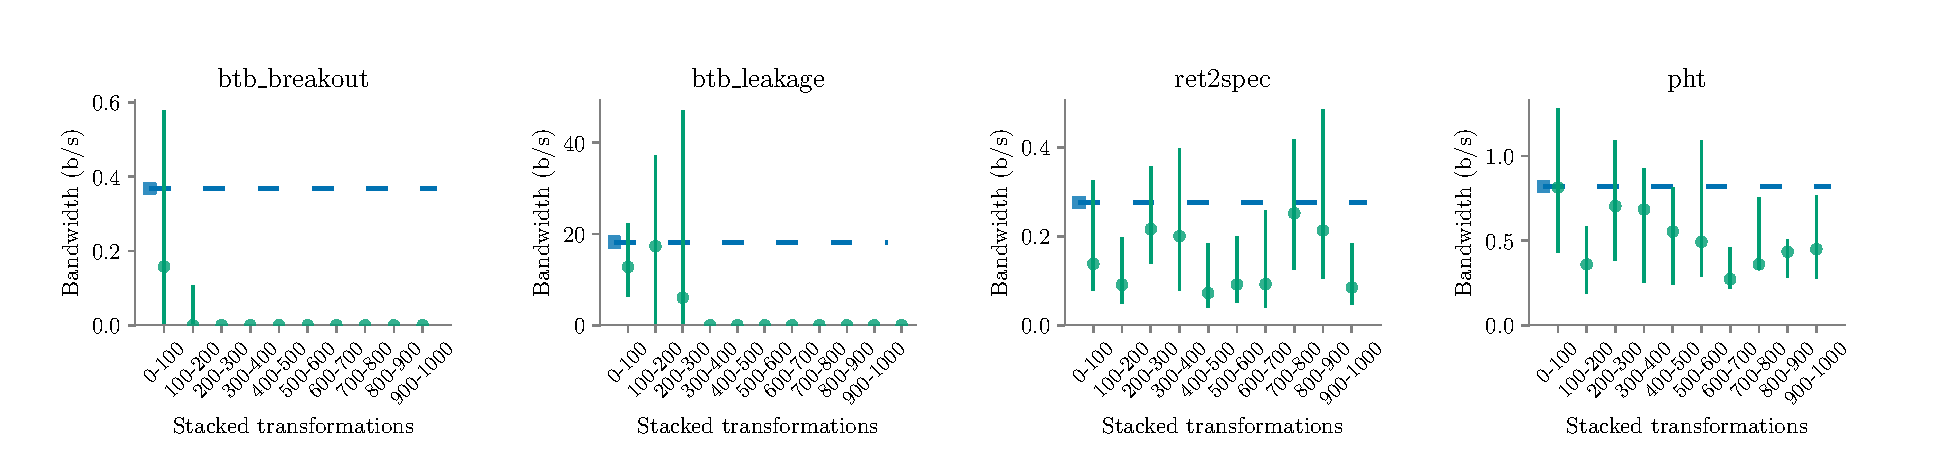
\includegraphics[width=\linewidth]{plots/rq3/results.rq3.pdf}
    \caption{Visual representation of \tool's impact on Swivel's original programs. The Y-axis denotes exfiltration bandwidth, with the original binary's bandwidth under attack highlighted by a blue marker and dashed line. Variants are clustered in groups of 100 stacked transformations, denoted by green dots (median bandwidth) and lines (interquartile bandwidth range). Overall, for all 100000 variants generated out of each original program, 70\% have less data leakage bandwidth.}
  \label{attacks:impact}
\end{figure*}

To answer \ref{rq:defensive}, we execute \tool on four distinct binaries \wasm susceptible to three Spectre attacks. Each of the four programs is subjected to a sequence of transformations with 100 different seeds. 
We stack up to 1000 transformations for each seed. 
At each juncture of the stacking process, we assess the resulting impact of the attacks as outlined in \ref{protocol:rq3}. 
The  analysis encompasses a total of 4$\times$100$\times$1000 binaries, which also includes the original four.

\autoref{attacks:impact} offers a graphical representation of \tool's influence on the Swivel original programs and their attacks. 
Each plot corresponds to one original \wasm binary and the attack it undergoes: btb\_breakout, btb\_leakage, ret2spec, and pht.
The Y-axis represents the exfiltration bandwidth (see \autoref{metric:ber}). 
The bandwidth of the original binary under attack is marked as a blue  dashed horizontal line.
In each plot, the variants are grouped in clusters of 100 stacked transformations. 
These are indicated by green dots and lines. 
The dot signifies the median bandwidth for the cluster, while the line represents the interquartile range of the group's bandwidth.



% General results for all cases
In the instances of btb\_breakout and btb\_leakage, \tool demonstrates a effectiveness, generating variants that leak less information than the original in 78\% and 70\% of the cases, respectively.
For these particular binaries, a significant reduction in exfiltration bandwidth to zero is noted following 200 stacked transformations across all 100 seeds.
As a result, with a minimum of 200 stacked transformations, \tool can create variants that are completely resistant to the original attack.
For the ret2spec and pht scenarios, the trend towards bandwidth reduction is less pronounced.
Nevertheless, the produced variants consistently exhibit lower bandwidth than the original in 76\% and 71\% of instances, respectively.
% Why is good, for breaking timers and for padding
As depicted in the plots, the exfiltration bandwidth diminishes following the application of 100 stacked transformations.

% High level of what we have seen
Our observations, articulated in response to \ref{rq:dynamic}, show that \tool fabricates variants that effectively alter memory access patterns. 
Specifically, it does so by amplifying spill/reload operations, instituting artificial global variables, and changing the frequency of pre-existing memory accesses. 
These transformations influence the \wasm program's memory, potentially causing disruption to any cache time predictors. 
As a result, these alterations contribute to a reduction in exfiltration bandwidth.

% More fine grained
On the other hand, many attacks rely on a timer component to measure cache access time for memory lines, and disrupting this component can effectively impair the attack's precision. 
This strategy of dynamic alteration has been purposefully employed in different scenarios. 
For instance, to counter potential timing attacks, Firefox randomizes its built-in JavaScript timer \cite{10.1007/978-3-319-70972-7_13}. \tool conveniently facilitates this strategy by interspersing instructions within the timing steps of \wasm variants. 
In \autoref{example:timer} and \autoref{example:timer2}, we demonstrate \tool's impact on time measurements. 
The former illustrates the original time measurement, while the latter presents a variant with \tool-inserted operations amid the timing.


\lstdefinestyle{watcode}{
  numbers=none,
  stepnumber=1,
  numbersep=10pt,
  tabsize=4,
  showspaces=false,
  breaklines=true, 
  showstringspaces=false,
    moredelim=**[is][{\btHL[fill=weborange!40]}]{`}{`},
    moredelim=**[is][{\btHL[fill=celadon!40]}]{!}{!}
}


   \begin{minipage}[b]{\linewidth}
    \lstset{
        language=WAT,
                        style=watcode,
        basicstyle=\footnotesize\ttfamily,
                        columns=fullflexible,
                        breaklines=true}
        
        \begin{lstlisting}[label=example:timer,caption={Wasm timer used in btb\_breakout program.},frame=b, captionpos=b]{Name}
;; Code from original btb_breakout
...
(call $readTimer)
(set_local $end_time)
... access to mem
(i64.sub (get_local $end_time ) (get_local $start_time))
(set_local $duration)
...

        \end{lstlisting}
\end{minipage}


\begin{minipage}[b]{\linewidth}
    \lstset{
        language=WAT,
                        style=watcode,
        basicstyle=\footnotesize\ttfamily,
                        columns=fullflexible,
                        breaklines=true}
        
        \begin{lstlisting}[label=example:timer2,caption={Variant of btb\_breakout with more instructions added in between time measurement.},frame=b, captionpos=b]{Name}
;; Variant code
...
(call $readTimer)
(set_local $end_time)
!<inserted instructions>!
... access to mem
!<inserted instructions>!
(i64.sub (get_local $end_time ) (get_local $start_time))
(set_local $duration)
...
        \end{lstlisting}
\end{minipage}


\tool proves effective against cache access timers because the time measurement of single or a few instructions is inherently random. 
By introducing more instructions, this randomness is amplified, thereby reducing the timer's accuracy.
% Mention something about performance here

%\todo{J: TBD, I was about to add a piece of code here, but the RQ is already too large. TODO }
Furthermore, CPUs have a maximum capacity for the number of instructions they can cache.
\tool integrates instructions in such a way that the vulnerable instruction may exceed this cacheable instruction limit.
This kind of transformation can be viewed as padding \cite{padding}.
In \autoref{example:padding} and \autoref{example:padding2}, we illustrate the effect of \tool on padding instructions.
\autoref{example:padding} presents the original code used for training the branch predictor, along with the expected speculated code.
Conversely, \autoref{example:padding2} showcases a variant where \tool embeds instructions within the memory accesses.


\lstdefinestyle{watcode}{
  numbers=none,
  stepnumber=1,
  numbersep=10pt,
  tabsize=4,
  showspaces=false,
  breaklines=true, 
  showstringspaces=false,
    moredelim=**[is][{\btHL[fill=weborange!40]}]{`}{`},
    moredelim=**[is][{\btHL[fill=celadon!40]}]{!}{!}
}


   \begin{minipage}[b]{0.9\linewidth}
    \lstset{
        language=WAT,
                        style=watcode,
        basicstyle=\footnotesize\ttfamily,
                        columns=fullflexible,
                        breaklines=true}
        
        \begin{lstlisting}[label=example:padding,caption={Two jump locations in btb\_breakout. The top one trains the branch predictor, the bottom one is the expected jump that exfiltrates the memory access.},frame=b, captionpos=b]{Name}
;; Code from original btb_breakout
...
;; train the code to jump here (index 1)
(i32.load (i32.const 2000))
(i32.store (i32.const 83)) ;; just prevent optimization
...
;; transiently jump here
(i32.load (i32.const 339968)) ;; S(83) is the secret
(i32.store (i32.const 83)) ;; just prevent optimization
        \end{lstlisting}
\end{minipage}


\begin{minipage}[b]{0.9\linewidth}
    \lstset{
        language=WAT,
                        style=watcode,
        basicstyle=\footnotesize\ttfamily,
                        columns=fullflexible,
                        breaklines=true}
        
        \begin{lstlisting}[label=example:padding2,caption={Variant of btb\_breakout with more instructions added indindinctly between jump places.},frame=b, captionpos=b]{Name}
;; Variant code
...
;; train the code to jump here (index 1)
!<inserted instructions>!
(i32.load (i32.const 2000))
!<inserted instructions>!
(i32.store (i32.const 83)) ;; just prevent optimization
...
;; transiently jump here
!<inserted instructions>!
(i32.load (i32.const 339968)) ;; "S"(83) is the secret
!<inserted instructions>!
(i32.store (i32.const 83)) ;; just prevent optimization
...
        \end{lstlisting}
\end{minipage}


The padding alters the arrangement of the binary code in memory, effectively impeding the attacker's capacity to initiate speculative execution.
Even when an attack is launched and the vulnerable code is "speculated", the memory access is not.


In every program, we note that the exfiltration bandwidth tends to be greater than the original when the variants include a small number of transformations.
This indicates that, although the transformations generally contribute to the reduction of data leakage, the initial few might not consistently contribute positively towards this objective.
We have identified several fundamental reasons, which we discuss below.

Firstly, as emphasized in prior applications of \tool \cite{CABRERAARTEAGA2023103296}, uncontrolled diversification can be counterproductive if a specific objective, such as a cost function, is not established at the beginning of the diversification process.
%Second, \tool applies certain "symmetric" transformations.
%In particular, vulnerable code segments may be duplicated across the variants, rendering the variant more susceptible to exploitation. 
%  For later \todo{these symmetric transformations also occur with large number of transformations, so why are the variants with many transformations protected?}
Secondly, while some transformations yield distinct \wasm binaries, their compilation produces identical machine code.
Transformations that are not preserved undermine the effectiveness of diversification.
% This is to answer to the RW of Swivel itself, they proposed ot add nop operations. We know that does not work.
For example, incorporating random \texttt{nop} operations directly into \wasm does not modify the final machine code as the \texttt{nop} operations are easily removed by the standard lucet compiler.
The same phenomenon is observed with transformations to custom sections of \Wasm binaries.
Additionally, it is important to note that transformed code doesn't always execute, i.e., \tool may generate dead code.

Finally, for ret2spec and pht, both exhibit a subtle trend towards bandwidth reduction, but this does not materialize in a short-term timeframe (low count of stacked transformations) when comparing to btb\_breakout and btb\_leakage.
Furthermore,  the exfiltration bandwidth is more dispersed for these two programs.
Our analysis indicates a correlation between these trends and the complexity of the binary subject to diversification.
Ret2spec and pht are considerably larger than btb\_breakout and btb\_leakage.
The former comprises more than 300k instructions, while the latter two include fewer than 800 instructions.
Given that \tool applies precise, fine-grained transformations one at a time, the likelihood of impacting critical attack components, such as timing memory accesses, diminishes for larger binaries, particularly when limited to 1,000 transformations.
Based on these observations, we believe that a greater number of stacked transformations will further contribute to completely eliminating the attacks associated with ret2spec and pht.

% Performance impact


%\todo{It might be possible to run a test-case reducer...would it work?}

%\todo{TBD: Someone might say that the performance is affected and that is why we have less bandwidth. The idea is to answer to this in RQ2. On the other hand, I have collected the times as well, we can show the execution time distribution in clusters.}

\begin{tcolorbox}[boxrule=1pt,arc=.3em,boxsep=-1.3mm]
  \textbf{Answer to \ref{rq:defensive}}:   software diversification is effective at synthesizing \wasm binaries that are less susceptible  to Spectre attacks.  
  \tool generates variants of btb\_breakout and btb\_leakage that are totally protected and variants of ret2spec and pht that are more resilient than the original.
Larger programs require a greater number of transformations to effectively neutralize Spectre attacks.
    In general, 70\% of of the diversified variants exhibit a reduced data leakage bandwidth compared to their original programs.
\end{tcolorbox}


%\todo{The complexity of the program affects the impact. The larger the program, more difficult to target specific locations. Notions of "knobs". Measure some meta of the original binaries. Number of functions, size in bytes, number of instructions. With more instructions, more the chances to hit the incorrect location.}




%\todo{the pht attack works better. It is more resilient. The reason is related to PHT. Pattern history table attach. Elaborate on this.}


%\todo{Add a figure to show how the traces change. Use tracergraph for it...it will be easier.}


%\tool


%\subsection{\rqtesting}

%\todo{We break binaryen...that is a good takeaway.}


%\todo{Variants generated with wasm-mutate break binaryen ! This might be case 3 !} \todo{We can collect the tools for Wasm presented along all these years and break them, highlighting the need for more testing...this will be nice.}


\section{Discussion}
\label{discussion}


\subsection{Preservation} 
\todo{we have not provided any number, so we should substantiate this with a claim }
The substantial differences in code preservation between JIT compilers carry notable implications. 
\todo{not a sentence}
For example, between wasmtime and V8.
On one side, high preservation rates signal a possible deficiency in optimizations, as previously underlined in \cite{wasmslim}. 
Conversely, high preservation may inadvertently allow vulnerable code to persist.
For instance, although \tool can generate more resilient variants, the compiler's role in mitigating initial vulnerabilities is crucial. 
High preservation could, therefore, potentially hinder the removal of potential security weaknesses during the compilation process.
\todo{subsection not convincing I would remove}


\subsection{Fuzzing \Wasm compilers with \tool}
\todo{interesting section but very unclear, tell the goal first. don't mention "seed"}
Identifying effective seeds for initiating fuzzing processes is a recognized challenge \cite{7958599}. 
\todo{Martin does not see the logical relationship between the first and second sentence}
However, programs known to be correctly compiled and executed can be diversified using \tool.
This research presents compelling evidence of preservation and variation in execution traces at an impressive scale, e.g., thousands of unique programs generated from a single original binary seed. 
As our analysis of preservation suggests, this strategy can effectively exert pressure on more compiler components, thereby enhancing the fuzzing coverage.



\subsection{Program Normalization}
\todo{this paragraph is not at all about wasm-mutate, remove}
\tool was previously employed successfully for the evasion of malware detection, as outlined in \cite{CABRERAARTEAGA2023103296}. 
The proposed mitigation in the prior study involved code normalization as a means of reducing the spectrum of malware variants. 
Our current work provides insights into the potential effectiveness of this approach. 
Specifically, a practically costless process of pre-compiling Wasm binaries could be employed as a preparatory measure for malware classifiers. 
In other words, a \wasm binary can first be compiled with wasmtime, effectively eliminating approx. 25\% of malware variants according to our preservation statistics for wasmtime. 
This approach could substantially enhance the efficiency and precision of malware detection systems.

\subsection{Mitigating Port Contention} 
Rokicki et al. \cite{10.1145/3488932.3517411} showed the practicality of a covert side-channel attack using port contention within \Wasm code in the browser. This attack fundamentally relies on the precise prediction of Wasm instructions that trigger port contention on specific ports.
To combat this security concern, we propose an man-in-the-middle mechanism, \tool, which could be conveniently implemented as a browser plugin. 
\tool has the ability to replace the \wasm instructions used as port contention predictor with other random instructions.
This will inevitably remove the port contention in the specific port used to conduct the attack.
\todo{not a sentence}
Thus, hardening browsers against such exploitative maneuvers.




\section{Related Work}
\label{rw}
% Binary Software diversification, static 
Static software diversification refers to the process of producing, synthesizing, and distributing unique but functionally equivalent binary files to end users. 
The implementation of this process can take place at any stage of software development and deployment - from the inception of source code, through the compilation phase, to the execution of the final binary \cite{jackson2011compiler, lundquist2016searching}.
\tool, a static diversifier, can be placed at the final stage, keeping in mind that the code will subsequently undergo final compilation by JIT compilers.
The concept of software diversification owes much to the pioneering work of Cohen \cite{cohen1993operating}. 
His suite of code transformations aimed to increase complexity and thereby enhance the difficulty of executing a successful attack against a broad user base \cite{cohen1993operating}. 
\tool's rewriting rules draw significantly from Cohen's seminal contributions.
Furthermore, Jackson and colleagues \cite{jackson2011compiler} proposed that the compiler can play a pivotal role in promoting static software diversification. 
Building on the previous idea, CROW is the only software diversification tool designed exclusively for \wasm. 
CROW's approach heavily incorporates prior techniques, as acknowledged by its creators \cite{arteaga2020crow}. 
Labelled as a superdiversifier \cite{jacob2008superdiversifier}, CROW positions the LLVM compiler as the central focus of its diversification method. 
However, the creators of CROW have also identified certain limitations.
For one, integrating the diversifier directly into the LLVM compiler, though not inherently problematic, restricts the tool's applicability to \wasm binaries generated through LLVM. 
This implies that any \wasm source code that lacks an LLVM frontend implementation cannot take advantage of CROW's capabilities.
In contrast, \tool adopts the same diversification techniques as CROW but provides a more versatile and faster \wasm to \wasm solution, maintaining compatibility with any compiler. 
Secondly, unlike CROW, \tool does not rely on an SMT solver to validate the generated variants. 
Instead, it guarantees semantic equivalence by design, resulting in greater efficiency in generating \wasm variants, as discussed in \autoref{rq:static:results}.
Lastly, \tool expands on CROW's capabilities by incorporating memory-like transformations. 
As a \wasm to \wasm diversification tool, \tool augments the range of tools capable of generating \wasm programs, a topic explored comprehensively throughout this work.

% For example, a custom rewriting rule could be  )
The process of diversifying a \Wasm program can be conceptualized as a three-stage procedure: parsing the program, transforming it, and finally re-encoding it back into \wasm. 
Our review of the literature has revealed several studies that have employed parsing and encoding components for \wasm binaries across various domains. 
This indicates that these works accept a \wasm binary as an input and output a unique \wasm binary. 
These domains span optimization \cite{wasmslim}, control flow \cite{10123627}, and dynamic analysis \cite{wasabi, stievenart2020compositional, 10123627, BRITO2022102745}.
When the transformation stage introduces randomized mutations to the original program, the aforementioned tools could potentially be construed as diversifiers \cite{some paper claming this}.
However, as they have been custom-built for specific tasks, these tools lack the necessary adaptability to function as all-purpose diversifiers. 
Interestingly, the other side of the coin is possible with \tool.
For instance, \tool can serve as both an optimizer and a test case reducer due to the incorporation of an e-graph at the heart of its diversification process \cite{10.1145/1480881.1480915}. 
To the best of our knowledge, the introduction of an e-graph into \tool marks the first endeavor to integrate an e-graph into a \wasm to \wasm analysis tool.



%\todo{and so what is the main conclusion here? that we could not reuse these tools for diversification? that  \tool could be used for some of these tasks? do some tools use e-graphs? is that the main novelty of \tool regarding wasm analysis?}

BREWasm \cite{rewritingtool2023} offers a comprehensive static binary rewriting framework for \Wasm and can be considered to be the most similar to \tool. 
For instance, it can be used to model a diversification engine.
It parses a Wasm binary into objects, rewrites them using fine-grained APIs, integrates these APIs to provide high-level ones, and re-encodes the updated objects back into a valid Wasm binary. 
The effectiveness and efficiency of BREWasm have been demonstrated through various Wasm applications and case studies on code obfuscation, software testing, program repair, and software optimization. 
%\todo{I do not understand the following 2 sentences. What are the main differences between \tool and BREWasm? in their input? in their output? in their purpose? in their technical approach? }
BREWasm implementation follows a completely different technical approach.
In comparison with our work, the authors pointed out that our tool employs lazy parsing of Wasm. 
Although they perceived this as a limitation, it is eagerly implemented to accelerate the generation of \wasm binaries.
Additionally, our tool leverages the parser and encoder of wasmtime, a standalone compiler and interpreter for Wasm, thereby boosting its reliability and lowering its error-prone nature.


\tool has previously been tested and proven successful for malware evasion \cite{CABRERAARTEAGA2023103296}.
Madvex \cite{madvex}, on the same topic, alters Wasm binaries with the goal of eluding malware detectors according to a generic reward function. 
Their approach primarily focuses on modifying the code section of an input Wasm binary. 
\tool demonstrates its capacity to employ a broader range of transformations, not confined solely to the code section.
Therefore, generating malware variants without affecting the code, and thus their performance.


\section{Conclusion}
\label{conc}

% We summarize the three RQs
\tool exhibits robust diversification, with a 100\% diversification rate across the original 303 programs proposed by CROW. 
It creates over 9000 unique variants per program in just an hour, boasting thousands of unique machine code variants, despite preservation rates of \preserved for the wasmtime JIT compiler, cranelift. 
These variants enable examination of compiler optimization impacts.
Despite non-preservation and dead code generation, \tool ensures significant diversity in execution traces. 
Moreover, \tool enhances resilience against Spectre attacks, producing fully protected variants of two versions of the btb attack, and variants of ret2spec and pht that leak less data than the original ones.


% Future work
In future works, we aim to fine-tune the diversification process, balancing broad diversification with the practical needs of real-world applications. 
The creation of rewriting rules for \tool is currently a manual task, yet we have identified potential for automation. 
For instance, \tool could be enhanced through incorporation of automatically verified rewriting rules, potentially sourced via data-driven methods such as rule mining from CROW \cite{10026577}.
Furthermore, we have observed that the impact of \tool on ret2spec and pht attacks is considerably less compared to btb attacks. 
These attacks exploit the returning address of executed functions in the program stack. 
As discussed in \ref{rq:dynamic}, \tool can generate variants that alter the return addresses of semantically equivalent functions. 
This suggests the potential for a multivariant execution strategy, similar to MEWE \cite{MEWE}, that can be implemented using \tool. 
By offering different execution paths, the returning addresses on the stack at each function execution would vary, thereby hardening binaries against ret2spec and pth attacks.
Overall, we plan striking a balance between code preservation, uniqueness of execution traces, and improved security of the generated variants.


\bibliographystyle{ACM-Reference-Format}
\bibliography{main}

\end{document}
\endinput
%%
%% End of file `sample-sigplan.tex'.


https://dl.acm.org/doi/pdf/10.1145/3547622